\documentclass{article}
\usepackage[utf8]{inputenc}
\usepackage[margin=2cm]{geometry}
\usepackage{amsmath, amssymb}
\usepackage{bm}
\usepackage{gensymb}
\usepackage{lineno}
\usepackage{lscape}
\renewcommand\linenumberfont{\normalfont\bfseries\small\color{darkgrey}}
\usepackage{booktabs}
\usepackage[round]{natbib}
\bibliographystyle{plainnat}
\usepackage{authblk}
% Linux Libertine:
\usepackage{textcomp}
\usepackage[sb]{libertine}
\usepackage[varqu,varl]{inconsolata}% sans serif typewriter
\usepackage[libertine,bigdelims,vvarbb]{newtxmath} % bb from STIX
\usepackage[cal=boondoxo]{mathalfa} % mathcal
\useosf % osf for text, not math
%\usepackage[supstfm=libertinesups,%
%  supscaled=1.2,%
%  raised=-.13em]{superiors}
\usepackage{setspace}
\usepackage{siunitx}
\usepackage[section]{placeins} % Keep floats (figs, tabs, eqns) in the right section
% I assume these all work together to make nice colour
\usepackage[dvipsnames]{xcolor}
\definecolor{niceblue}{HTML}{236899} % Depends \usepackage[dvipsnames]{xcolor}
\definecolor{darkgrey}{HTML}{A9A9A9} % Depends \usepackage[dvipsnames]{xcolor}
% End nice colour
\usepackage{pgfplotstable} % For tables
\pgfplotsset{compat=1.16} % For tables
\newcommand{\yearStart}{1979}
\newcommand{\yearEnd}{2017}
\newcommand{\nYears}{39}
\newcommand{\nRegionsThree}{3}
\newcommand{\nRegionsSix}{6}
\newcommand{\nRegionsEight}{8}
\newcommand{\nReleased}{881205}
\newcommand{\nReleasedAK}{358074}
\newcommand{\nReleasedBC}{485262}
\newcommand{\nReleasedCC}{37869}
\newcommand{\nRecovered}{61906}
\newcommand{\nRecoveredAK}{17028}
\newcommand{\nRecoveredBC}{42456}
\newcommand{\nRecoveredCC}{42456}
\newcommand{\rawNReleased}{945332}
\newcommand{\rawNReleasedAK}{381129}
\newcommand{\rawNReleasedBC}{524720}
\newcommand{\rawNReleasedCC}{39483}
\newcommand{\rawNRecovered}{114780}
\newcommand{\rawNRecoveredAK}{40316}
\newcommand{\rawNRecoveredBC}{69737}
\newcommand{\rawNRecoveredCC}{4727}
\newcommand{\rawDaysDurationMin}{1}
\newcommand{\rawDaysDurationMean}{1224}
\newcommand{\rawDaysDurationMax}{13581}
\newcommand{\rawDistanceMin}{0}
\newcommand{\rawDistanceMean}{345}
\newcommand{\rawDistanceMax}{4806}
\newcommand{\daysDurationMin}{90}
\newcommand{\releasedSizeMin}{400}
\newcommand{\releasedSizeMax}{800}
\newcommand{\releasedSizeSmallMin}{400}
\newcommand{\releasedSizeSmallMax}{549}
\newcommand{\releasedSizeLargeMin}{550}
\newcommand{\releasedSizeLargeMax}{800}
\newcommand{\muNaturalMortality}{0.1}
\newcommand{\sdNaturalMortality}{0.01}
\newcommand{\muInitialLossRate}{0.1}
\newcommand{\sdInitialLossRate}{0.01}
\newcommand{\muOngoingLossRate}{0.02}
\newcommand{\sdOngoingLossRate}{0.001}
\newcommand{\muReportingRateAK}{0.4}
\newcommand{\muReportingRateBC}{0.5}
\newcommand{\muReportingRateCC}{0.3}
\newcommand{\sdReportingRateAK}{0.04}
\newcommand{\sdReportingRateBC}{0.05}
\newcommand{\sdReportingRateCC}{0.03}
\newcommand{\nChains}{1}
\newcommand{\stepSize}{0.01}
\newcommand{\adaptDelta}{0.95}
\newcommand{\iterWarmup}{250}
\newcommand{\iterSampling}{1000}
\newcommand{\maxTreedepth}{10}
\newcommand{\threadsPerChain}{5}

\usepackage{graphicx}
\graphicspath{ {./figs/} }
% hyperref must be last in preamble
\usepackage{hyperref}
\hypersetup{
    colorlinks=true,
    linkcolor=black,
    filecolor=black,      
    urlcolor=niceblue,
    citecolor=niceblue,
    linkbordercolor = white
}

% Title
\title{Sablefish movement and abundance exchange in the northeast Pacific: insights from four decades of tagging}

% Authors
\author[1]{Luke A. Rogers}
\author[]{...}

%Affiliations
\affil[1]{Pacific Biological Station, Fisheries and Oceans Canada, Nanaimo, BC, V9T 6N7, Canada}

\begin{document}

\maketitle
\linenumbers
\setcounter{secnumdepth}{0}

\section{Co-authorship}
Co-authorship and final author order to follow the PSTAT Data Sharing and Collaboration Agreement (\href{https://docs.google.com/document/d/1AXIhq6lO_qOPf7q67s_SiDOD6qEfih0COtxQZo7v-Hc/edit?usp=sharing}{here}).

\section{Abstract}

\section{Introduction}

\section{Methods}

\subsection{Data}

\subsection{Movement model}

\noindent Note: needs updates to language, possibly symbols (C to Q; s to lambda; theta to W?) 

We modeled sablefish movement as a hidden Markov process \cite[][]{langrock-2012-flexible-practical} observed nby tag recoveries. Sablefish entered the model as counts of tag releases identified by release region, time-step, and size class. The time-step in our analysis was one quarter-year. For a given release time-step and size class, the initial abundances of tagged sablefish were represented by a square diagonal matrix 

% Survival
\begin{equation}
  \label{eq:abundance-initial}
  \mathrm{diag} \! \left[\boldsymbol{A}_{i,d=1,l}\right] = \boldsymbol{R}_{i,l} \left(1 - \nu \right)
\end{equation}


where row corresponded to release region and diagonal elements were counts of tags released in each region diminished by the initial tag loss rate $\upsilon$. Subsequent tag abundances from the same release time-step and size class were defined recursively as 

% Abundance
\begin{equation}
    \label{eq:abundance}
    \boldsymbol{A}_{i,d,l} = \boldsymbol{A}_{i,d-1,l} \, \boldsymbol{\Gamma}_{n[i,d-1],l}
\end{equation}

\noindent where $n$ was some time-step after release, $\boldsymbol{\Gamma}_n$ acted as a transition matrix, and $\boldsymbol{A}_n$ encoded the projected tag abundances at the beginning of time-step $n$ with rows indicating the release region and columns indicating the destination region. 

What we refer to as the transition matrix $\boldsymbol{\Gamma}_n$ combined survival and movement rates as the matrix product

% Transition
\begin{equation}
    \label{eq:transition}
    \boldsymbol{\Gamma}_{n,l} = \boldsymbol{S}_{n,l} \, \boldsymbol{\Delta}_{l}
\end{equation}

\noindent where $\boldsymbol{S}_t$ was a diagonal matrix of step-wise survival rates in year $t$, $\boldsymbol{\Delta}_t$ was a square matrix of step-wise movement rates in year $t$, and $t[n]$ indexed year as a function of model step. While $\boldsymbol{\Delta}_t$ was a proper right stochastic matrix in the sense that its elements were probabilities and rows summed to one, $\boldsymbol{\Gamma}_n$ was not, because mortality removed some tagged sablefish from the model during each time-step. Consequently, mortality (including tag loss) formed an absorbing Markov state that could not be departed, in addition to the eight discrete non-absorbing states defined by the management regions. We chose to encode the mortality state implicitly via removal for clarity rather than assign an additional row and column to $\boldsymbol{\Gamma}_n$, and we refer to $\boldsymbol{\Gamma}_n$ as a transition matrix for convenience with the understanding that its rows did not sum to one.

Sablefish survival rates depended on mortality and tag loss as

% Survival
\begin{equation}
  \label{eq:survival}
  \mathrm{diag} \! \left[\boldsymbol{S}_{n,l}\right] = 
    \exp\!{\left[-\boldsymbol{s}_l \boldsymbol{f}_n - \boldsymbol{m} - \eta \right]}
\end{equation}

\noindent where $\boldsymbol{f}_n$ and $\boldsymbol{m}$ were row vectors of step-wise fishing and natural mortality, and $\eta$ was step-wise ongoing tag loss including tag-induced mortality. 

We modeled expected tag recoveries by the matrix product of tagged sablefish abundance and a step-wise observation rate. For a given release time-step and size class this was defined as

% Expected
\begin{equation}
  \label{eq:expected}
  \boldsymbol{\widehat{C}}_{i,d,l} = \boldsymbol{A}_{i,d,l} \boldsymbol{B}_{n[i,d],l}
\end{equation}

\noindent where $\boldsymbol{\widehat{C}}_{i,d,l}$ was a square matrix of expected tag recoveries with rows indicating release region and columns indicating recovery region, and $\boldsymbol{B}_{n,l}$ was a diagonal matrix of observation rates defined by the element-wise vector product

% Observation
\begin{equation}
  \label{eq:observation}
  \mathrm{diag} \! \left[\boldsymbol{B}_{n,l}\right] = 
    \boldsymbol{\theta} \left(1 - \exp\!{\left[-\boldsymbol{s}_l \boldsymbol{f}_{n} \right]} \right) 
\end{equation}

\noindent where $\boldsymbol{\theta}$ was a row vector of per-tag reporting rates and $\boldsymbol{f}_n$ was a vector of step-wise fishing mortality rates.

For a given release size class, we defined annual sablefish movement rates by a matrix power of the corresponding step-wise movement rates

% Movement rate
\begin{equation}
    \label{eq:movement}
    \boldsymbol{P}_{l} = \boldsymbol{\Delta}_{l}^K
\end{equation}

\noindent where $\boldsymbol{P}_{l}$ was the square matrix of annual movement rates, and $K$ was the number of time-steps per year.

% The matrix of step-wise movement rate deviations $\boldsymbol{\Lambda}_t = \boldsymbol{\Delta}_t - \boldsymbol{\bar{\Delta}}$ from the step-wise mean movement rates $\boldsymbol{\bar{\Delta}}$ was constrained by an autoregressive process on its diagonal

% Timevary
%\begin{equation}
%  \label{eq:timevary}
%  \mathrm{diag}\!\left[\boldsymbol{\Lambda}_t\right] = \mathrm{diag}\!\left[\boldsymbol{\Lambda}_{t-1}\right]\! \boldsymbol{\Psi} + \boldsymbol{\epsilon}_t, \, \boldsymbol{\epsilon}_t \sim \mathrm{N}\!\left[\boldsymbol{0},\,\boldsymbol{\Sigma}_\Lambda\right]
%\end{equation}

%\noindent where $\boldsymbol{\Psi}$ was a diagonal matrix of autocorrelation coefficients, and $\boldsymbol{\Sigma}_\Lambda$ was a diagonal variance matrix.

We used the NB2 parameterization of the negative binomial distribution with probability mass function

% Sampling
\begin{equation}
  \label{eq:sampling}
  \mathrm{NB2} \! \left[ C_* \mid \widehat{C}_*,\, \phi \right] = \binom{C_* + \phi - 1}{C_*} \left(\frac{\widehat{C}_*}{\widehat{C}_* + \phi}\right)^{C_*} \left( \frac{\phi}{\widehat{C}_* + \phi} \right)^{\phi}
\end{equation}

\noindent where $C_*$ and $\widehat{C}_*$ were the observed and expected tag recovery counts corresponding to a given release region, time-step and length class, and recovery region and time-step.

\subsection{Model fitting}

\subsection{Abundance exchange}

\subsection{Sensitivity analyses}

\section{Results}

\subsection{Movement rates}

\subsection{Abundance exchange}

\subsection{Sensitivity analyses}

\section{Discussion}

\section{Acknowledgements}

\section{Figures}

% map-regions-6-network
\begin{figure}[htb]
    \centering
    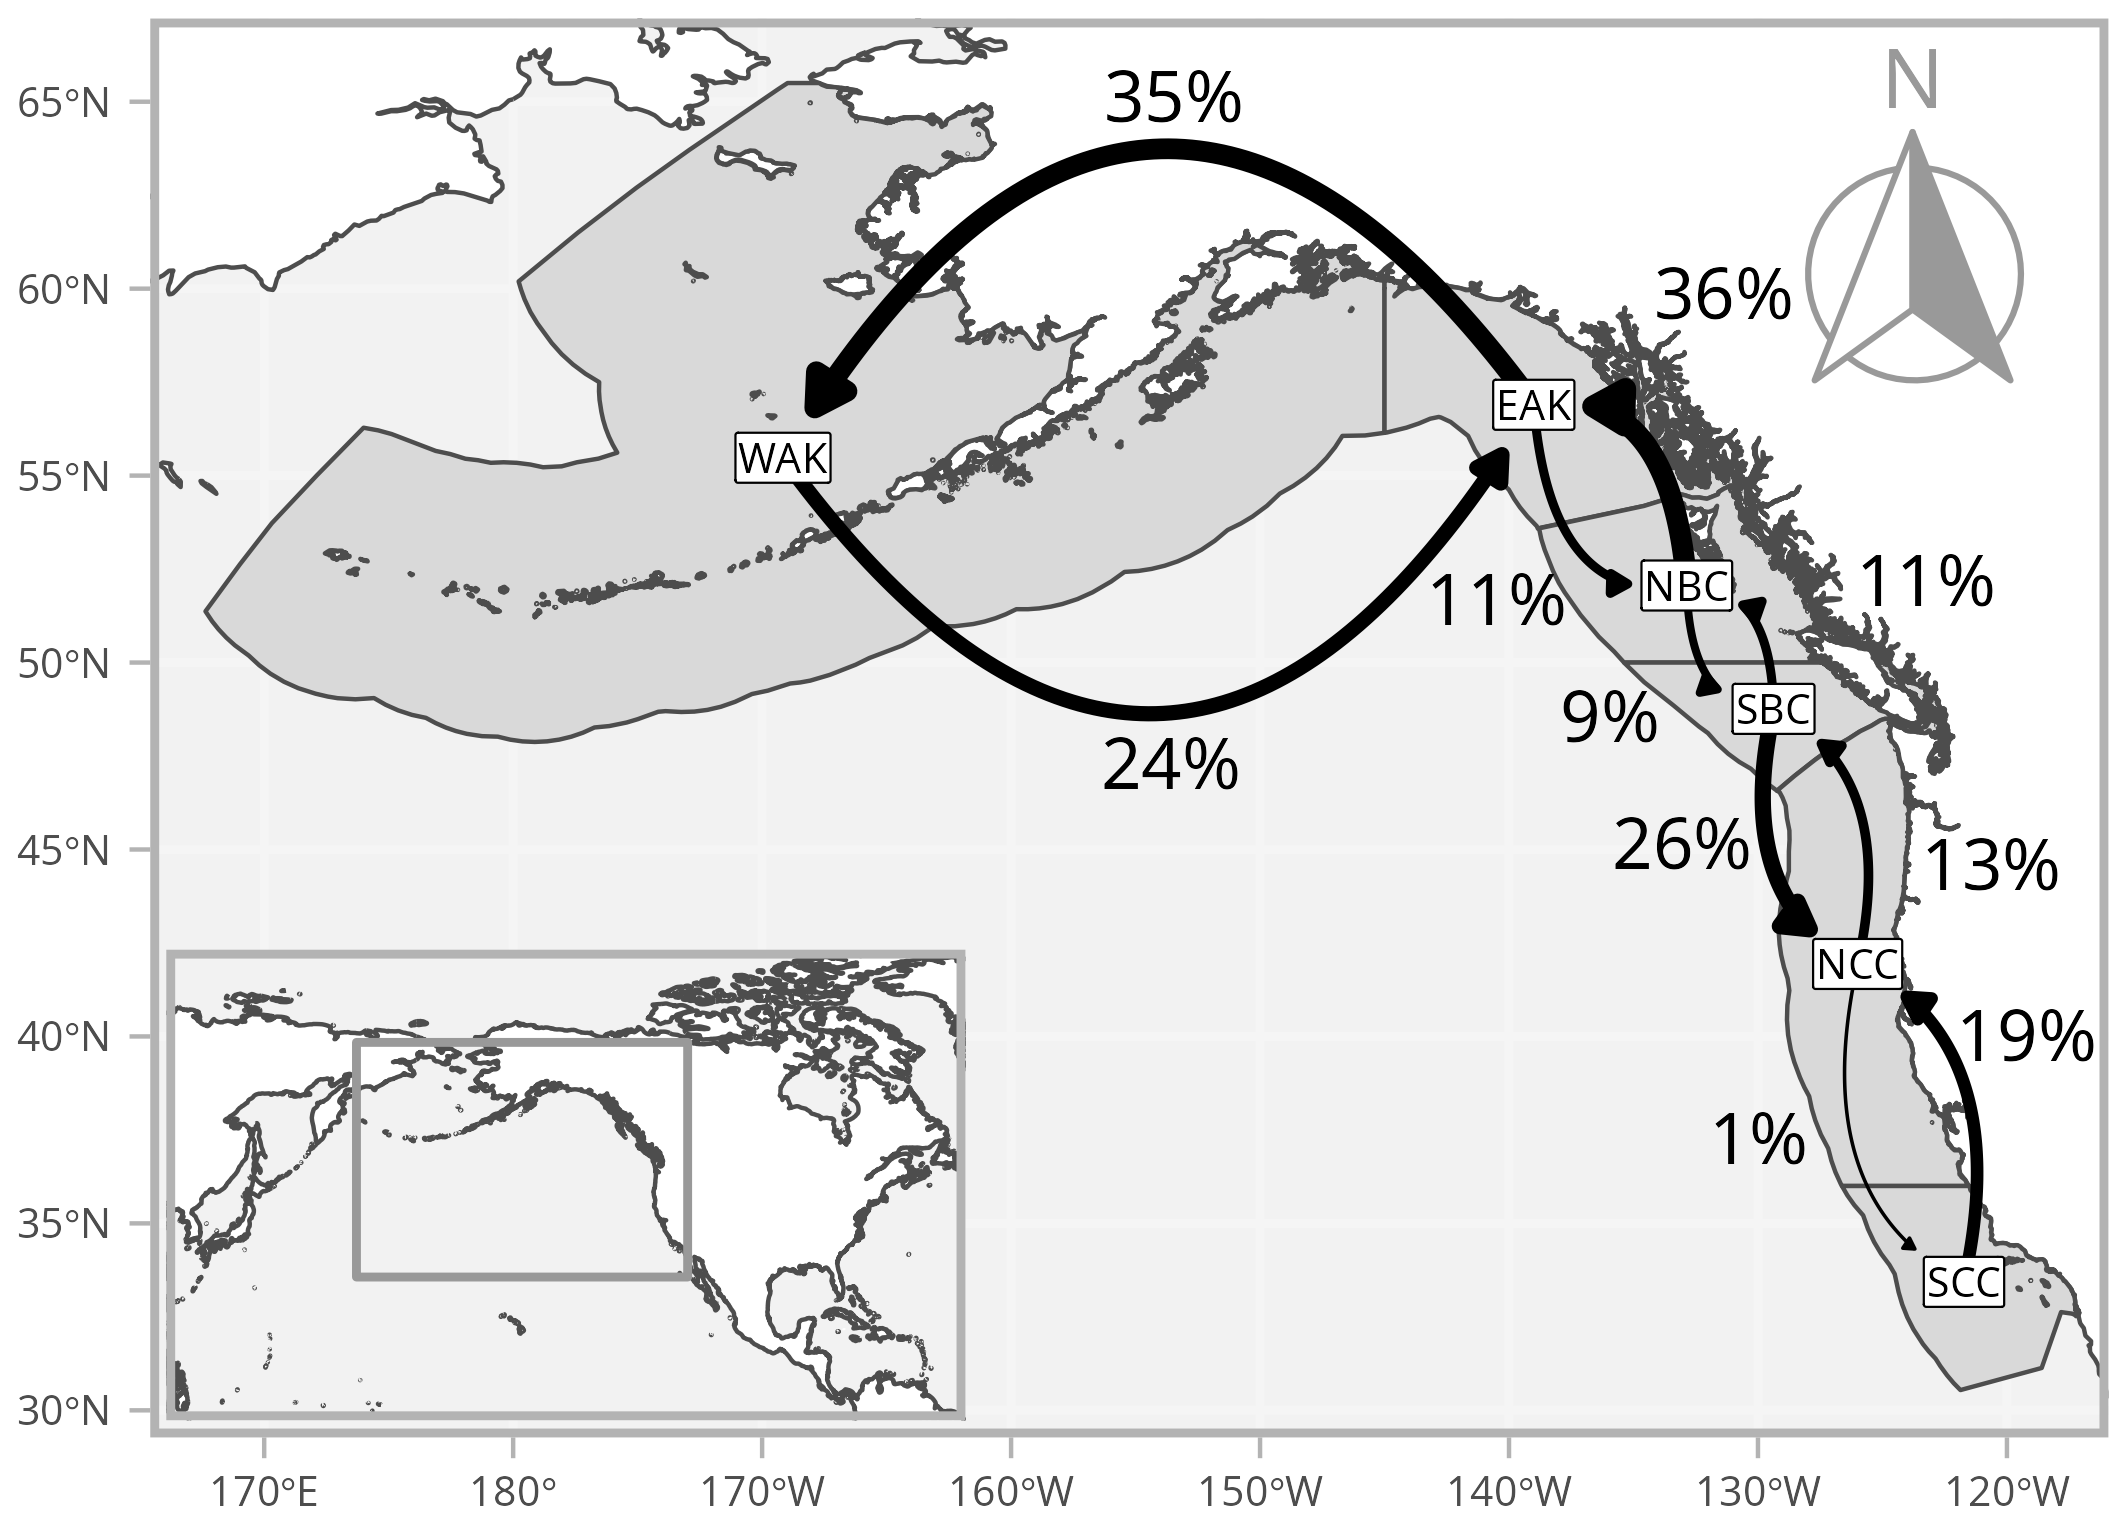
\includegraphics[width = 0.7\textwidth]{map-regions-6-network}
    \caption{Annual sablefish movement rates among six biogeographic regions in the northeast Pacific Ocean. Shown are 1\degree{} (between neighbouring regions: black arrows) percentage movement rates (per fish per year). WAK: West Alaska; EAK: East Alaska; NBC: North British Columbia; SBC: South British Columbia; NCC: North California Current; SCC: South California Current.}
    \label{fig:map-network-regions-6}
\end{figure}

\begin{figure}[htb]
    \centering
    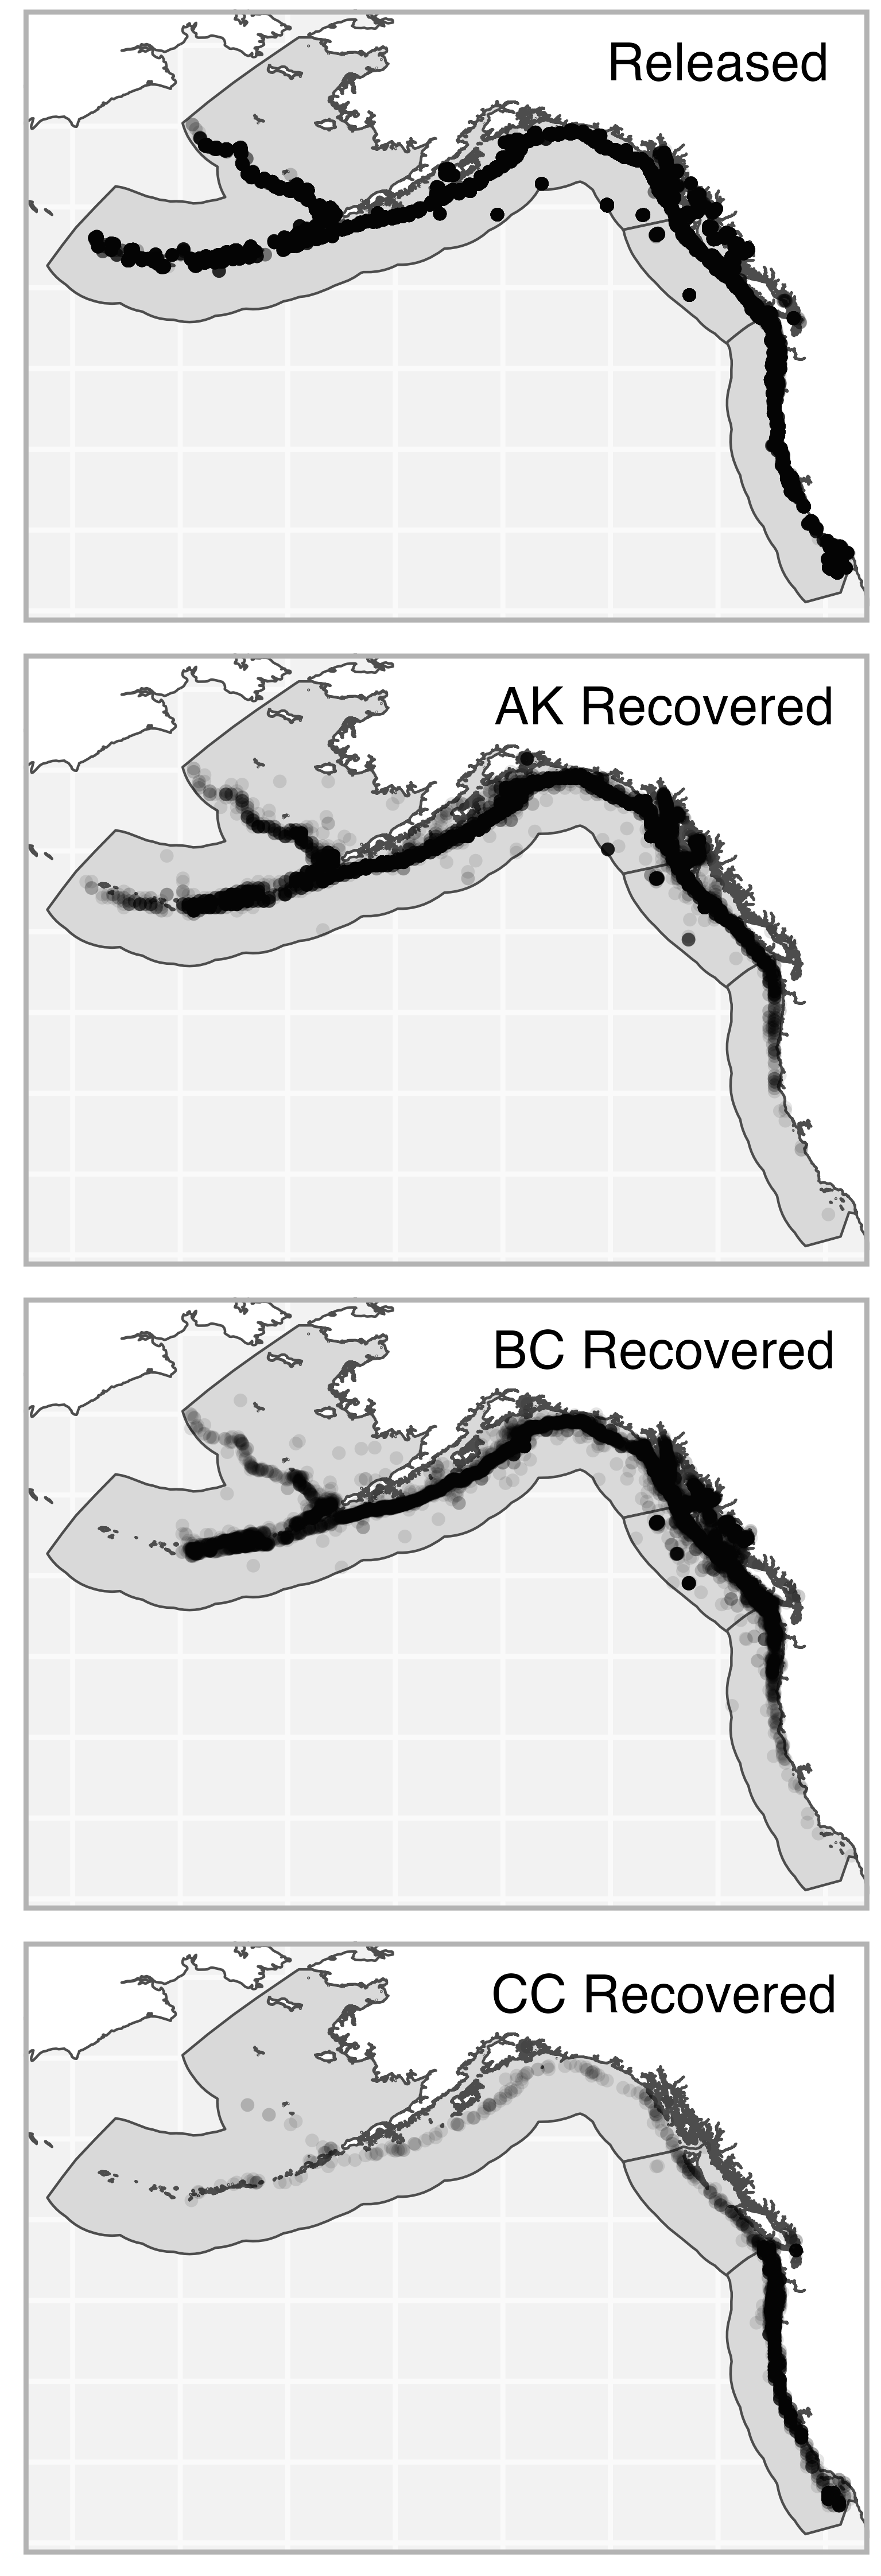
\includegraphics[width = 0.4\textwidth]{map-regions-3-released-recovered}
    \caption{Tagged sablefish released (top panel; coastwide) and recovered (bottom three panels by jurisdiction released) during 1979--2018. AK: Alaska; BC: British Columbia; CC: California Current.}
    \label{fig:map-regions-3-released-recovered}
\end{figure}

\begin{figure}[htb]
    \centering
    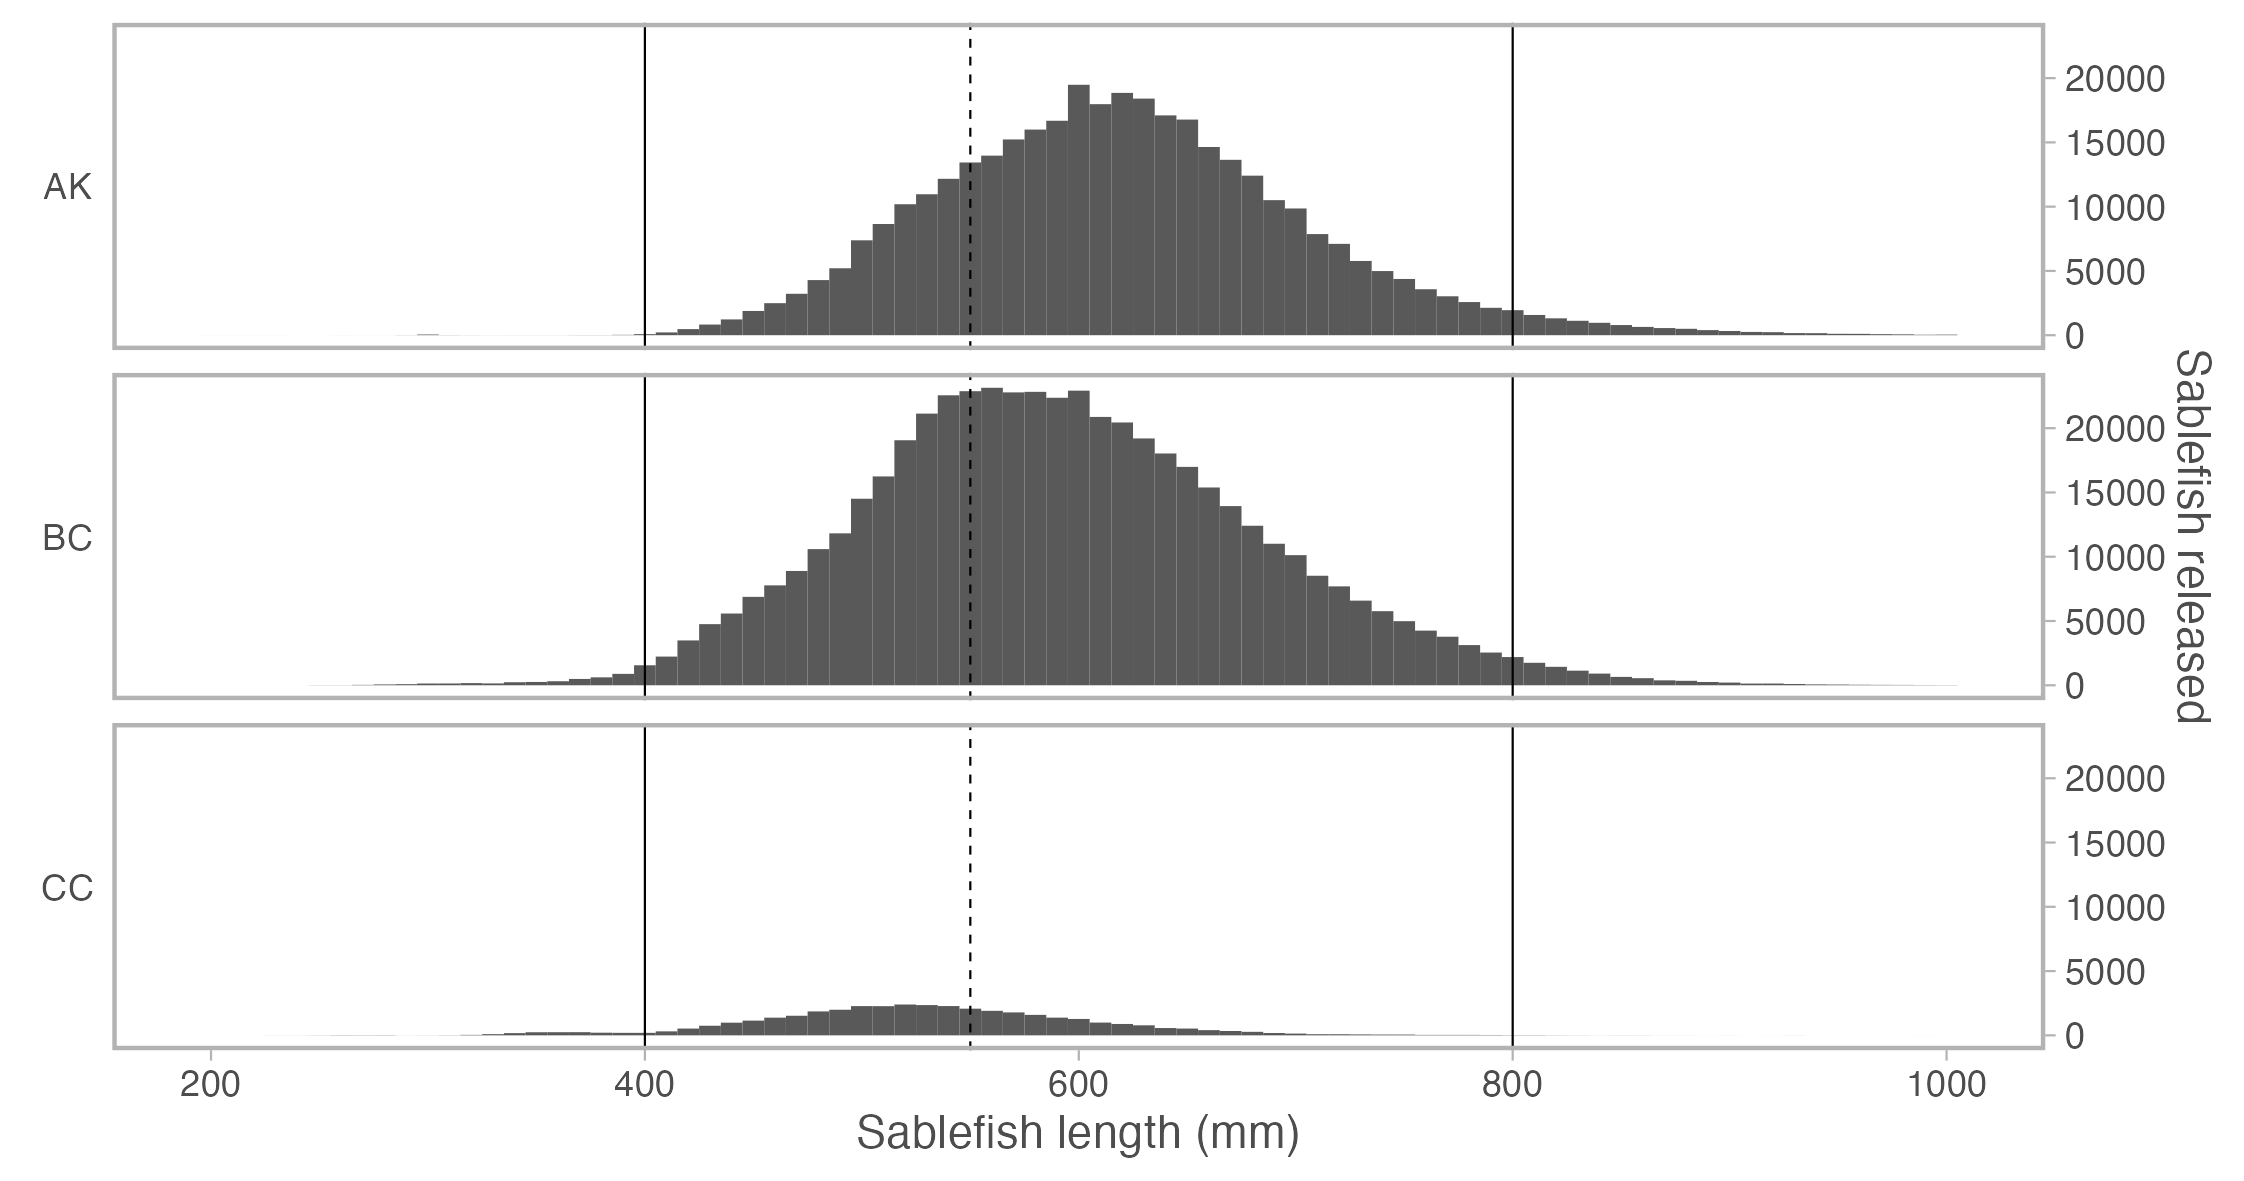
\includegraphics[width = 0.7\textwidth]{bar-regions-3-released-by-size}
    \caption{Sablefish released length (fork length: mm) by jurisdiction. AK: Alaska; BC: British Columbia; CC: California Current. Vertical lines show minimum and maximum sablefish length included in the study (solid lines; 400--800 mm) and division between small and large sablefish size classes (dashed line; 550 mm).}
    \label{fig:bar-regions-3-released-by-size}
\end{figure}

\begin{figure}[htb]
    \centering
    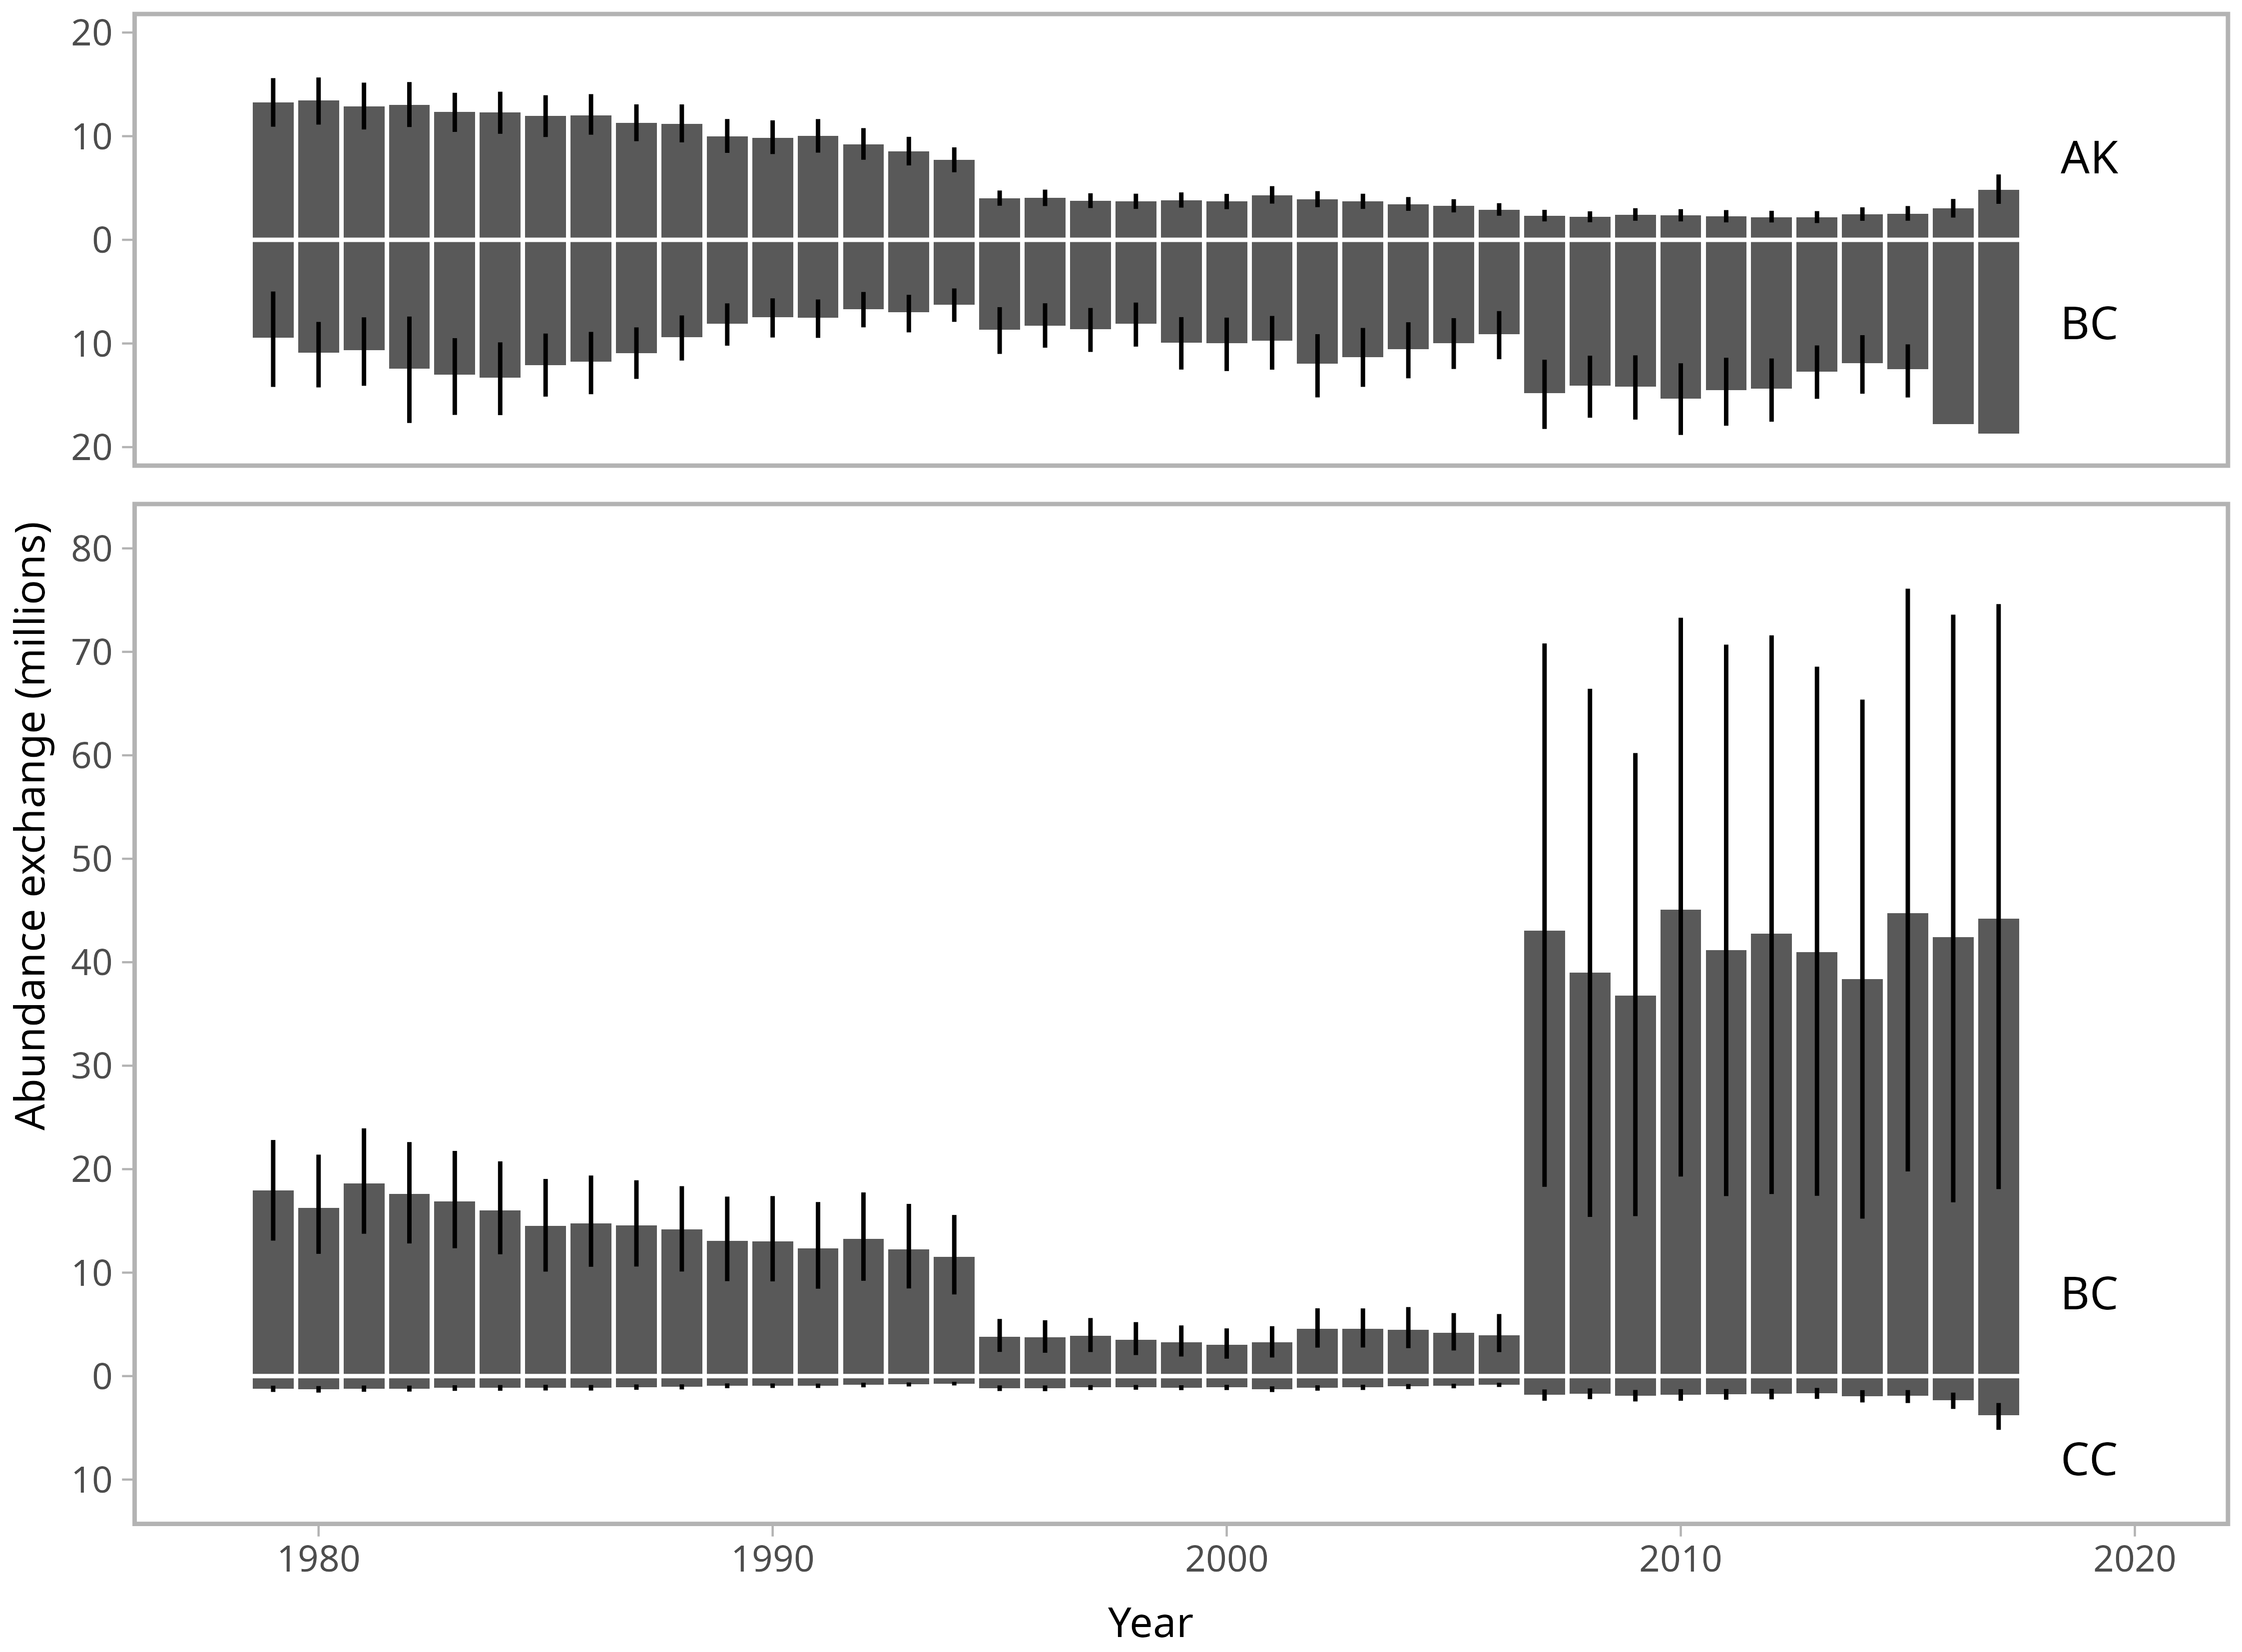
\includegraphics[width = 0.7\textwidth]{bar-abundance-exchange}
    \caption{Sablefish abundance exchange (millions; 90\%{} CI) between jurisdictions estimated from annual 1\degree{} movement rates with uncertainty and numbers of fish (age 2+) with uncertainty. Annual movement rates were estimated by year block: 1979--1994; 1995--2006; 2007--2017. Top panel: sablefish movement from BC to AK (above horizontal axis) and from AK to BC (below horizontal axis). Bottom panel: sablefish movement from CC to BC (above horizontal axis) and from BC to CC (below horizontal axis). AK: Alaska; BC: British Columbia; CC: California Current.}
    \label{fig:bar-abundance-exchange}
\end{figure}

\begin{figure}[htb]
p    \centering
    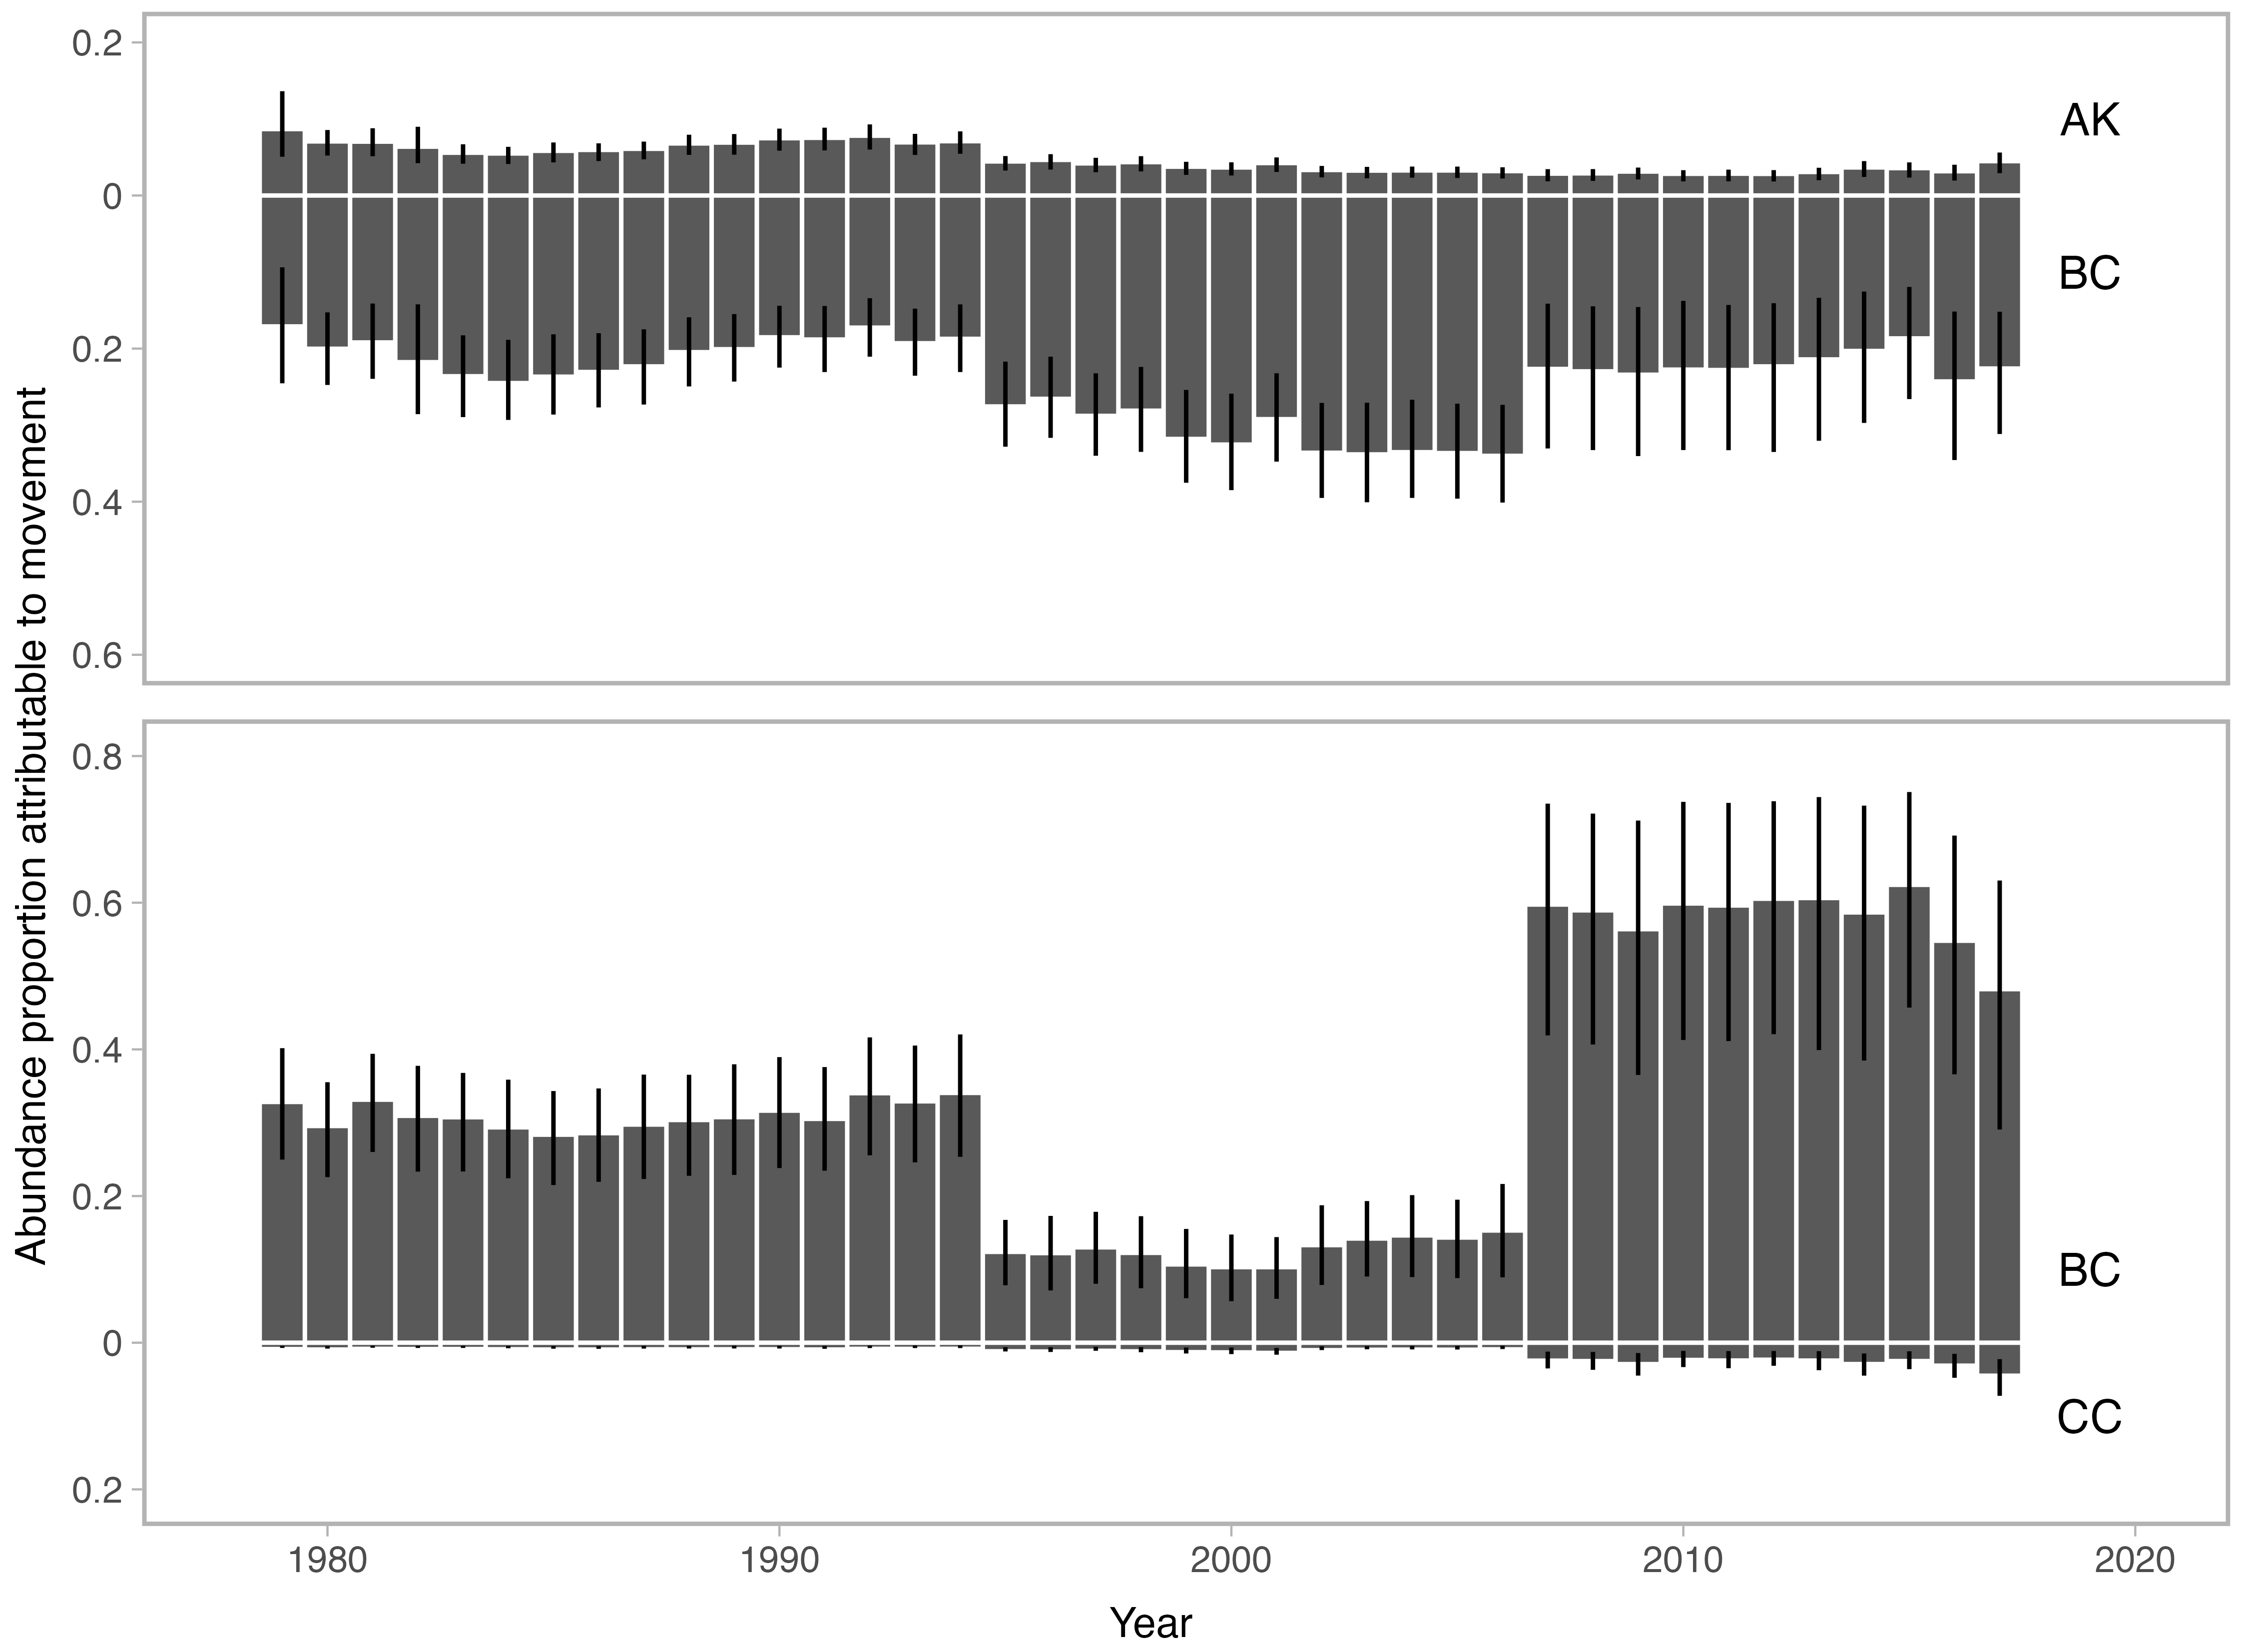
\includegraphics[width = 0.7\textwidth]{bar-percent-attributable}
    \caption{Proportion of sablefish abundance (90\%{} CI) within jurisdiction attributable to 1\degree{} movement between jurisdictions. Estimated from annual numbers of fish (age 2+) with uncertainty and annual movement rates with uncertainty. Annual movement rates were estimated by year block: 1979--1994; 1995--2006; 2007--2017. Top panel: proportion of numbers of sablefish in AK attributable to movement from BC (above horizontal axis) and proportion in BC attributable to movement from AK (below horizontal axis). Bottom panel: proportion of numbers of sablefish in BC attributable to movement from CC (above horizontal axis) and proportion in CC attributable to movement from BC (below horizontal axis). AK: Alaska; BC: British Columbia; CC: California Current.}
    \label{fig:bar-percent-attributable}
\end{figure}

\section{Tables}


\begin{table}[h]
  \begin{center}
  \caption{Sablefish mean annual movement rates (per fish per year; 90\%{} CI) between six biogeographic regions in the northeast Pacific Ocean. WAK: West Alaska; EAK: East Alaska; NBC: North British Columbia; SBC: South British Columbia; NCC: North California Current; SCC: South California Current.}
  \label{tab:movement-rate-regions-6-mean}
    \pgfplotstabletypeset[
      col sep=comma,                       % Commas separate .csv values
      columns/{0}/.style={column name={}}, % Replace autofilled column name by " "
      string type                          % Expect characters
    ]{tabs/movement-rate-regions-6-mean.csv}
  \end{center}
\end{table}


% Model indexes
\begin{table}[ht]
  \centering
  \caption{Movement model indexes}
  \renewcommand\arraystretch{1.2}
  \label{tab:model-indexes}
  \begin{tabular}{l l l l r}
    \toprule
    \textbf{Symbol} & \textbf{Condition} & \textbf{Dimension} & \textbf{Definition} & \textbf{Type} \\
    \toprule
    % Index limits
    $X$ & $\in \mathbb{Z}^{+}$ & Scalar & Number of geographic regions & Index limit \\
    $T$ & $\in \mathbb{Z}^{+}$ & Scalar & Number of years & Index limit \\
    $K$ & $\in \mathbb{Z}^{+}$ & Scalar & Number of time steps per year & Index limit \\
    $N$ & $ = TK $ & Scalar & Number of time steps & Index limit \\
    $D$ & $\in \mathbb{Z}^{+}$ & Scalar & Maximum time steps at liberty & Index limit \\
    $L$ & $\in \mathbb{Z}^{+}$ & Scalar & Number of release size classes & Index limit \\
    \midrule
    % Index variables
    $x, \, y$ & $\in \left[1 \, .. \, X \right]$ & Scalar & Geographic region & Index \\
    $t$ & $\in \left[1 \, .. \, T \right]$ & Scalar & Year & Index \\
    $n$ & $\in \left[1 \, .. \, N \right]$ & Scalar & Time step & Index \\
    $i$ & $\in \left[1 \, .. \, N\!-\!1 \right]$ & Scalar & Release time step & Index \\
    $k$ & $\in \left[1 \, .. \, K \right]$ & Scalar & Time step within year & Index \\
    $d$ & $\in \left[1 \, .. \, D \right]$ & Scalar & Time step at liberty & Index \\
    $l$ & $\in \left[1 \, .. \, S \right]$ & Scalar & Release size class & Index \\
    \bottomrule
  \end{tabular}
\end{table}

% Data
\begin{table}[ht]
  \centering
  \caption{Data}
  \renewcommand\arraystretch{1.2}
  \label{tab:data}
  \begin{tabular}{l l l l r}
    \toprule
    \textbf{Symbol} & \textbf{Condition} & \textbf{Dimension} & \textbf{Definition} & \textbf{Type} \\
    \toprule
    $\bm{R}$ & $\in \mathbb{Z}^{+,0}$ & $[N\!-\!1, L][X]$ & Sablefish tags released (counts) & Stepwise \\
    $\bm{C}$ & $\in \mathbb{Z}^{+,0}$ & $[N\!-\!1, D, L][X, X]$ & Sablefish tags recovered (counts) & Stepwise \\
    \bottomrule
  \end{tabular}
\end{table}

% Model derived quantities
\begin{table}[ht]
  \centering
  \caption{Movement model derived quantities}
  \renewcommand\arraystretch{1.2}
  \label{tab:model-derived}
  \begin{tabular}{l l l l r}
    \toprule
    \textbf{Symbol} & \textbf{Condition} & \textbf{Dimension} & \textbf{Definition} & \textbf{Type} \\
    \toprule
    $\bm{A}$ & $\in \mathbb{R}^{+,0}$ & $[N\!-\!1, D, L][X, X]$ & Sablefish tag abundance (numbers) & Stepwise \\
    $\boldsymbol{\widehat{C}}$ & $\in \mathbb{R}^{+,0}$ & $[N\!-\!1, D, L][X, X]$ & Sablefish expected tags recovered (numbers) & Stepwise \\
    $\boldsymbol{\Gamma}$ & $\in \left[0, 1 \right]$ & $[N, L][X, X]$ & Sablefish transition rates & Stepwise \\
    $\bm{S}$ & $\in \left[0, 1 \right]$ & $[N, L][X, X]$ & Sablefish survival rates & Stepwise \\
    $\bm{B}$ & $\in \left[0, 1 \right]$ & $[N, L][X]$ & Sablefish tag observation rates & Stepwise \\
    \midrule
    $\bm{P}$ & $\in \left[0, 1 \right]$ & $[L][X, X]$ & Sablefish movement rates & Annual \\
    $\bm{F}$ & $\in \mathbb{R}^{+,0}$ & $[T, X]$ & Sablefish instantaneous fishing mortality rates & Annual \\
    $\bm{M}$ & $\in \mathbb{R}^{+,0}$ & $[T, X]$ & Sablefish instantaneous natural mortality rates & Annual \\
%    \midrule
%    $\boldsymbol{\Lambda}$ & $\in \left[0, 1 \right]$ & $[L][X, X]$ & Sablefish movement rate deviations & Stepwise \\    
    \bottomrule
  \end{tabular}
\end{table}


% Model parameters
\begin{table}[ht]
  \centering
  \caption{Movement model parameters}
  \renewcommand\arraystretch{1.2}
  \label{tab:model-parameters}
  \begin{tabular}{l l l l r}
    \toprule
    \textbf{Symbol} & \textbf{Condition} & \textbf{Dimension} & \textbf{Definition} & \textbf{Type} \\
    \toprule
    $\boldsymbol{\Delta}$ & $\in \left[0, 1 \right]$ & $[L][X, X]$ & Sablefish movement rates & Stepwise \\
    $\bm{f}$ & $\in \mathbb{R}^{+,0}$ & $[N, X]$ & Sablefish instantaneous fishing mortality rates & Stepwise \\
    $\bm{s}$ & $\in \left[0, 1 \right]$ & $[L, X]$ & Sablefish fisheries size selectivity & Per fish \\
    $\bm{m}$ & $\in \mathbb{R}^{+,0}$ & $[X]$ & Sablefish instantaneous natural mortality rates & Stepwise \\
    $\boldsymbol{\theta}$ & $\in \left[0, 1 \right]$ & $[X]$ & Sablefish tag reporting rates & Per tag \\
    $\eta$ & $\in \mathbb{R}^{+,0}$ & Scalar & Sablefish instantaneous ongoing tag loss rate & Stepwise \\
    $\nu$ & $\in \left[0, 1 \right]$ & Scalar & Sablefish initial tag loss rate & Per tag \\    
    $\phi$ & $\in \mathbb{R}^{+}$ & Scalar & Negative binomial dispersion & NB2 \\
%    \midrule
    \bottomrule
  \end{tabular}
\end{table}






\section{Supplementary information}

\subsection{Supplementary figures}

\begin{figure}[htb]
    \centering
    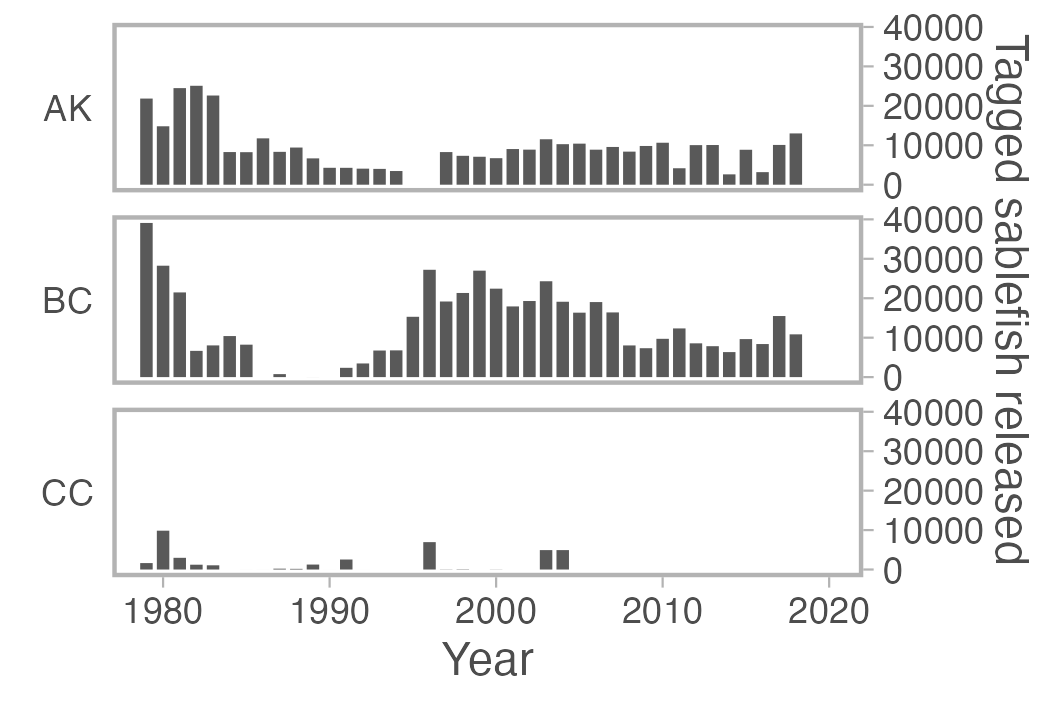
\includegraphics[width = 0.4\textwidth]{bar-regions-3-released-by-year}
    \caption{Number of tagged sablefish released by jurisdiction by year. AK: Alaska; BC: British Columbia; CC: California Current.}
    \label{fig:bar-regions-3-released-by-year}
\end{figure}

\begin{figure}[htb]
    \centering
    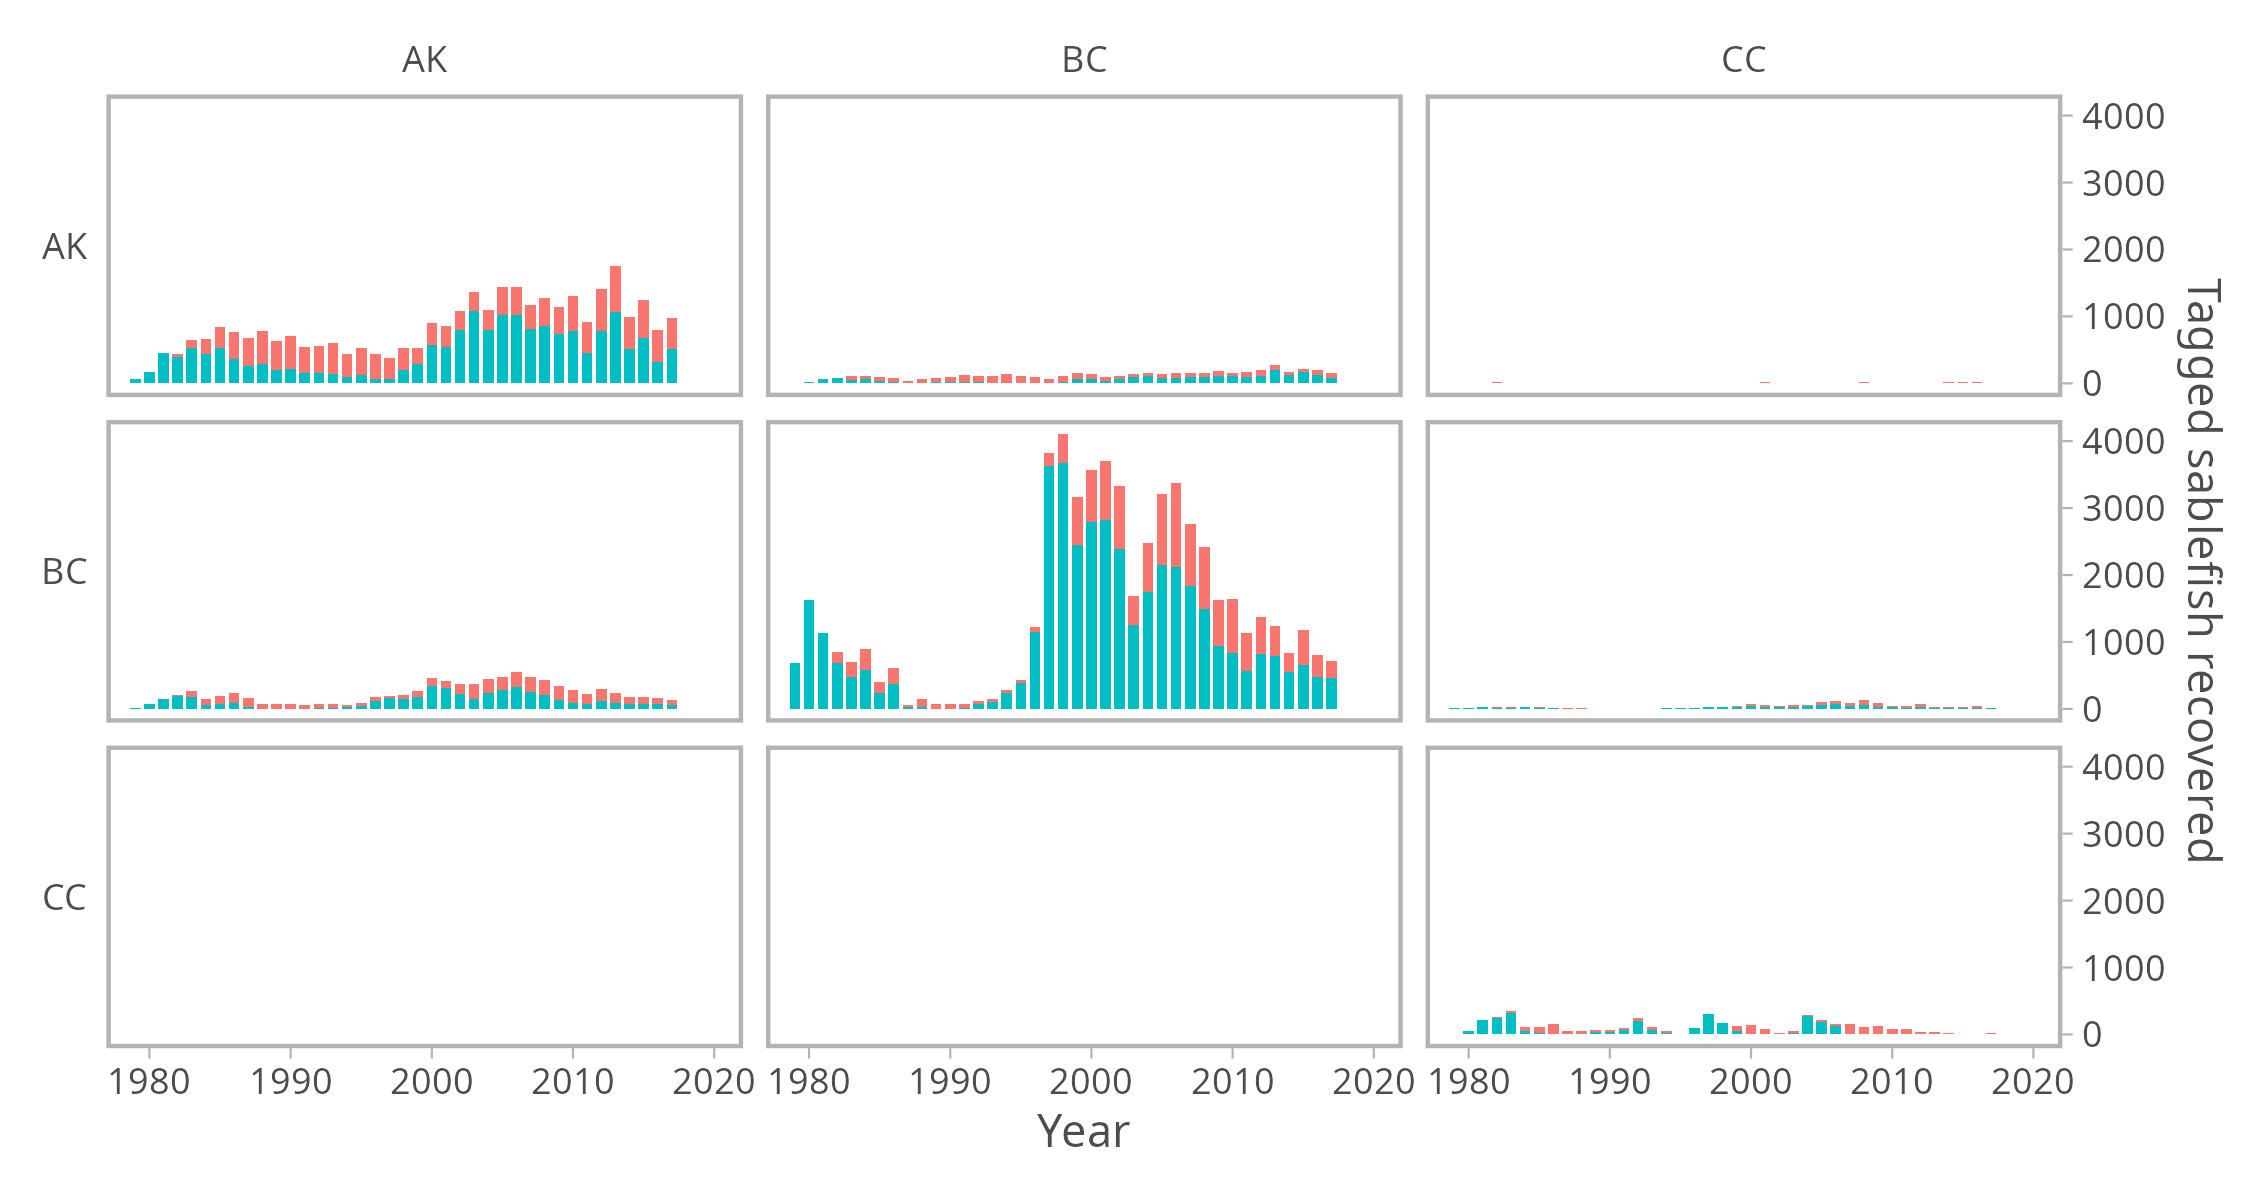
\includegraphics[width = 0.7\textwidth]{bar-regions-3-recovered-by-year}
    \caption{Number of tagged sablefish recovered by jurisdiction released (panel rows) and jurisdiction recovered (panel columns) by year. Green: recovered within 3 years of release; Orange: recovered more than three years after release. AK: Alaska; BC: British Columbia; CC: California Current.}
    \label{fig:bar-regions-3-recovered-by-year}
\end{figure}

\begin{figure}[htb]
    \centering
    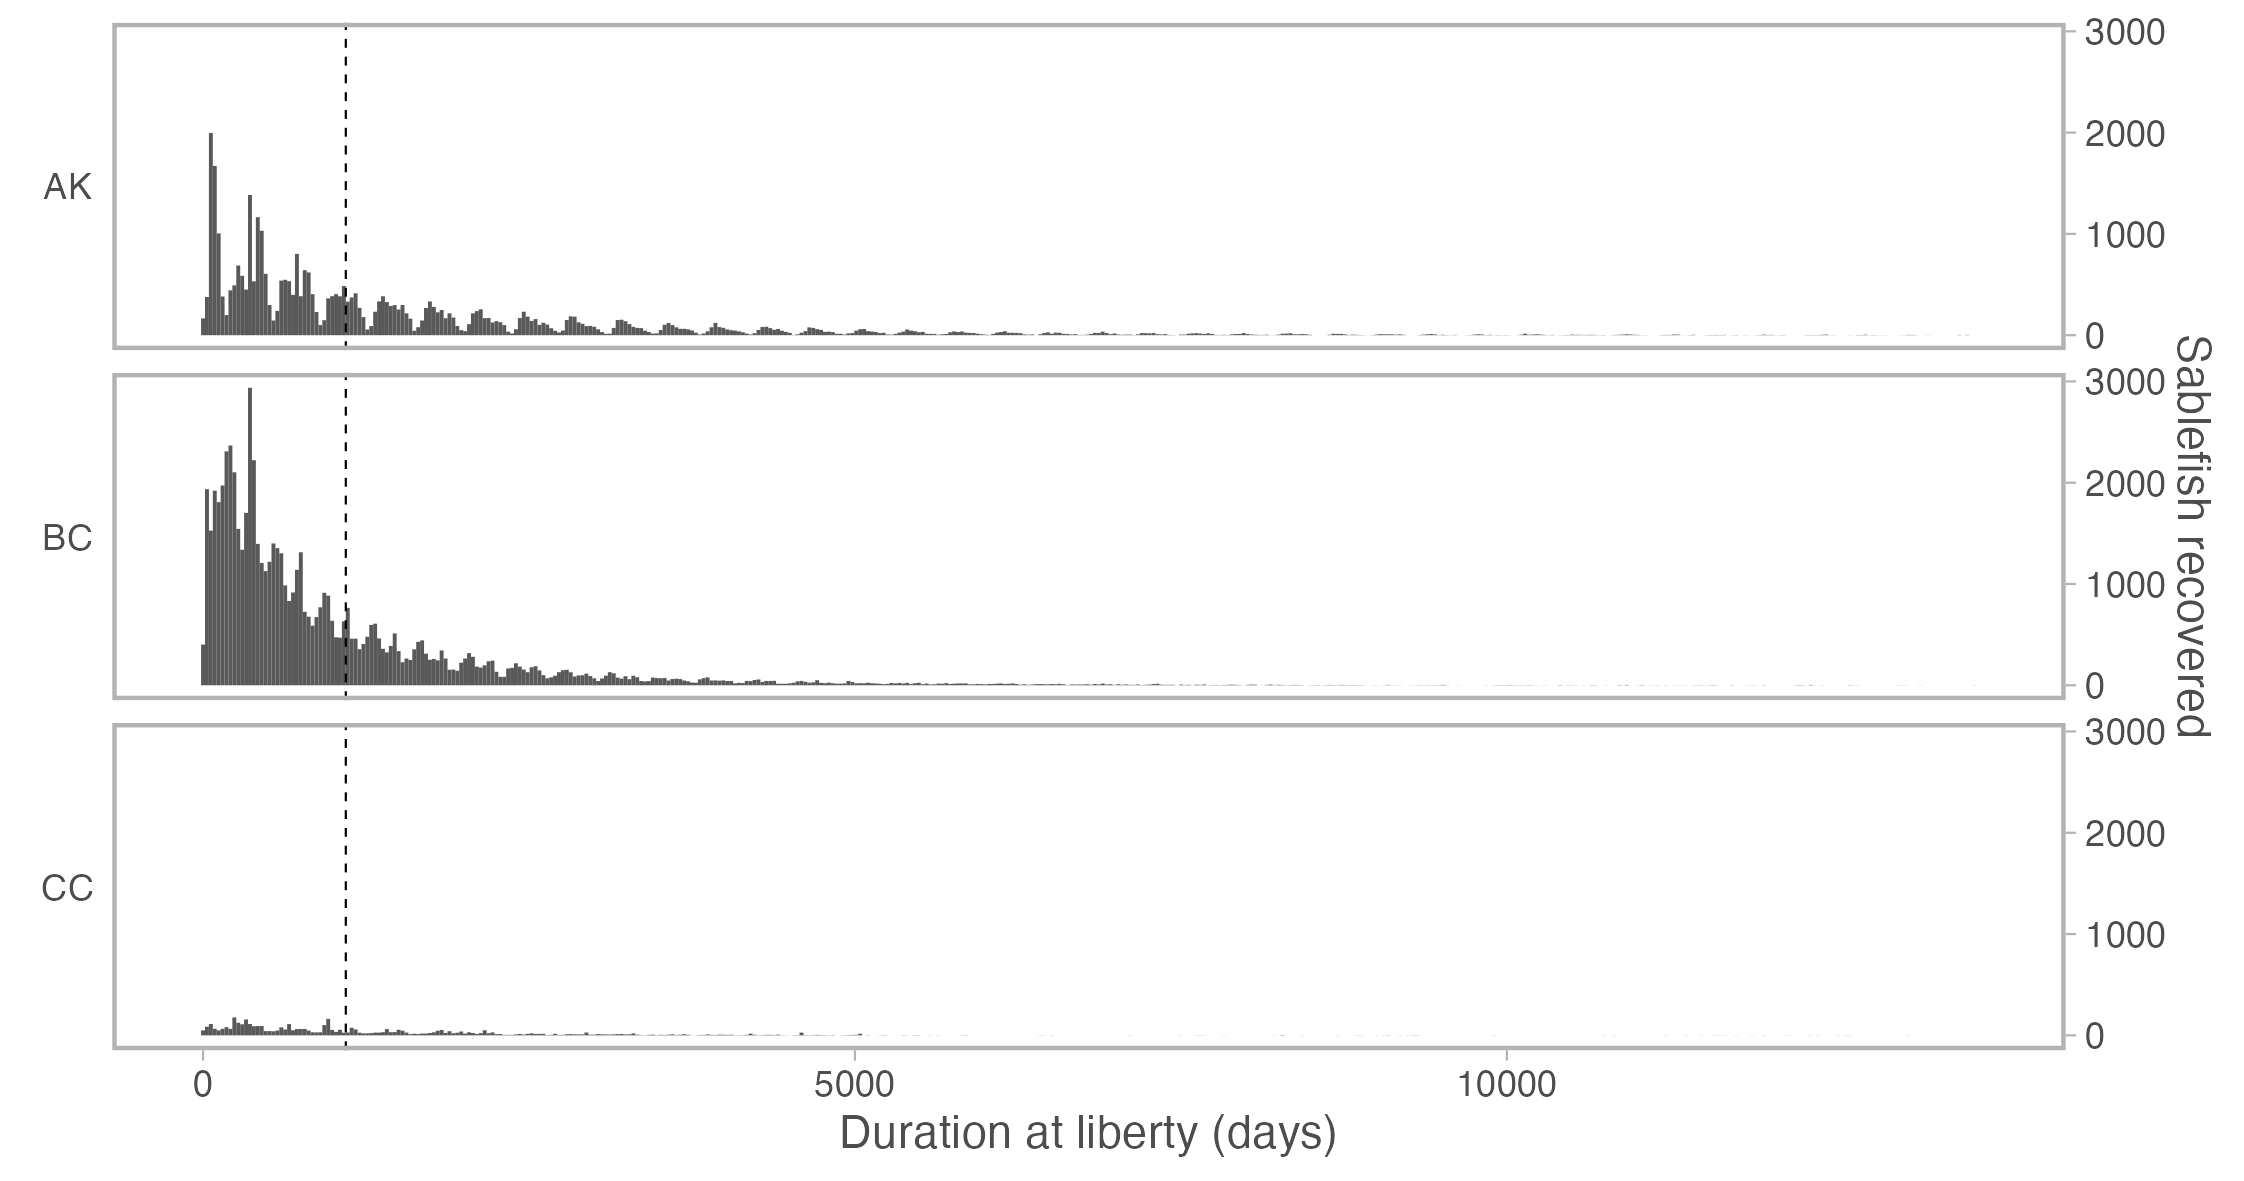
\includegraphics[width = 0.7\textwidth]{bar-regions-3-duration-at-liberty}
    \caption{Number of tagged sablefish recovered by jurisdiction released (panel rows) and duration at liberty (days) between date released and recovered. Dashed line: 3 years duration at liberty. AK: Alaska; BC: British Columbia; CC: California Current.}
    \label{fig:bar-regions-3-duration-at-liberty}
\end{figure}

\begin{figure}[htb]
    \centering
    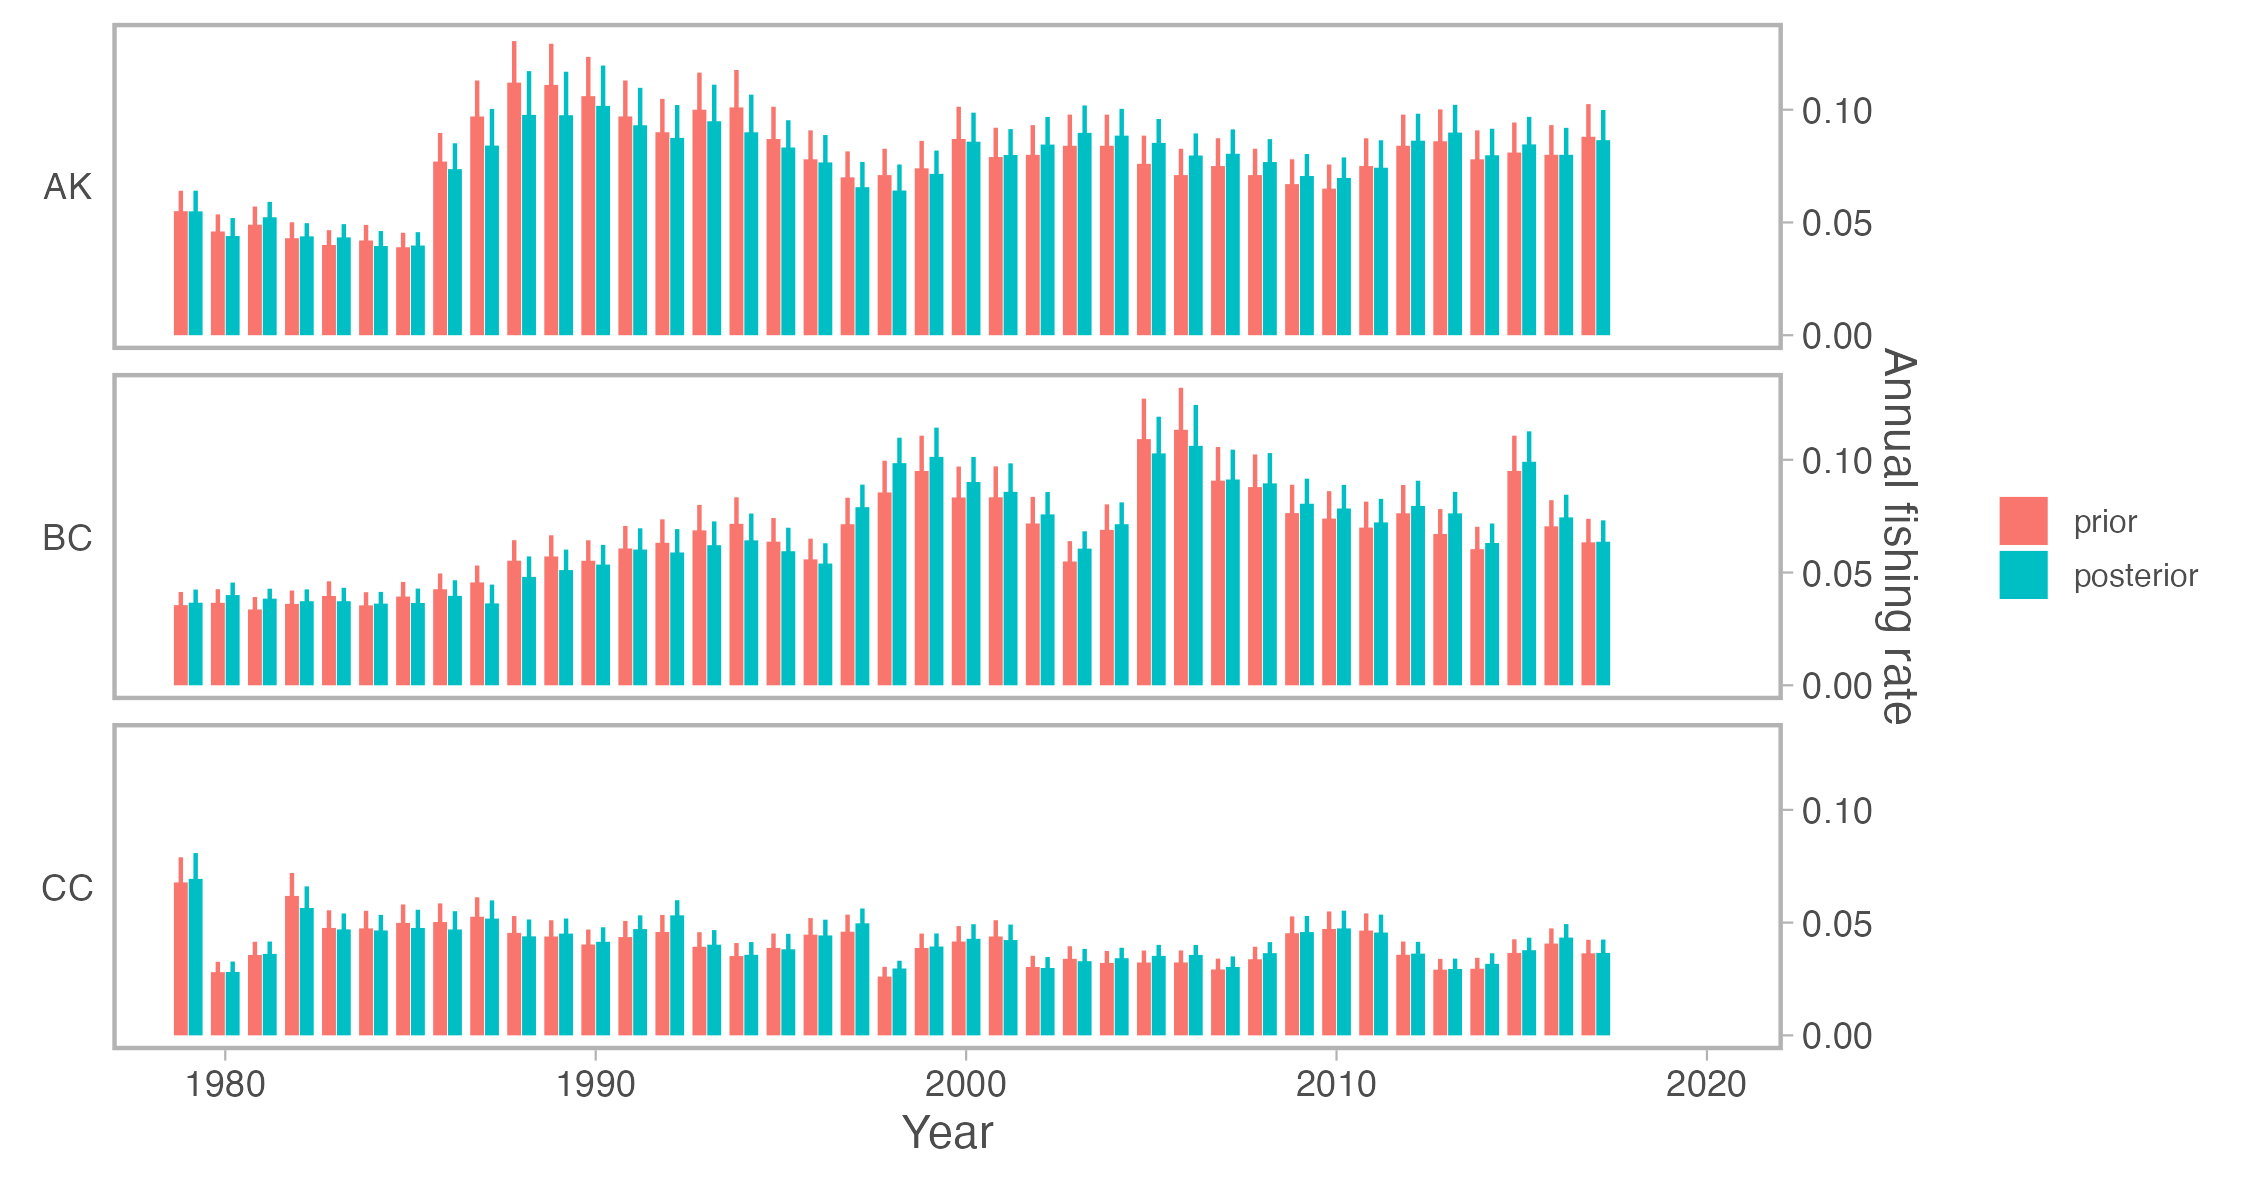
\includegraphics[width = 0.7\textwidth]{bar-regions-3-fishing-priors-posteriors}
    \caption{Sablefish annual fishing mortality rate prior and posterior means (90\% CI) by jurisdiction by year. Orange bars: prior means; teal bars: posterior means. AK: Alaska; BC: British Columbia; CC: California Current.}
    \label{fig:bar-regions-3-fishing-priors-posteriors}
\end{figure}

\begin{figure}[htb]
    \centering
    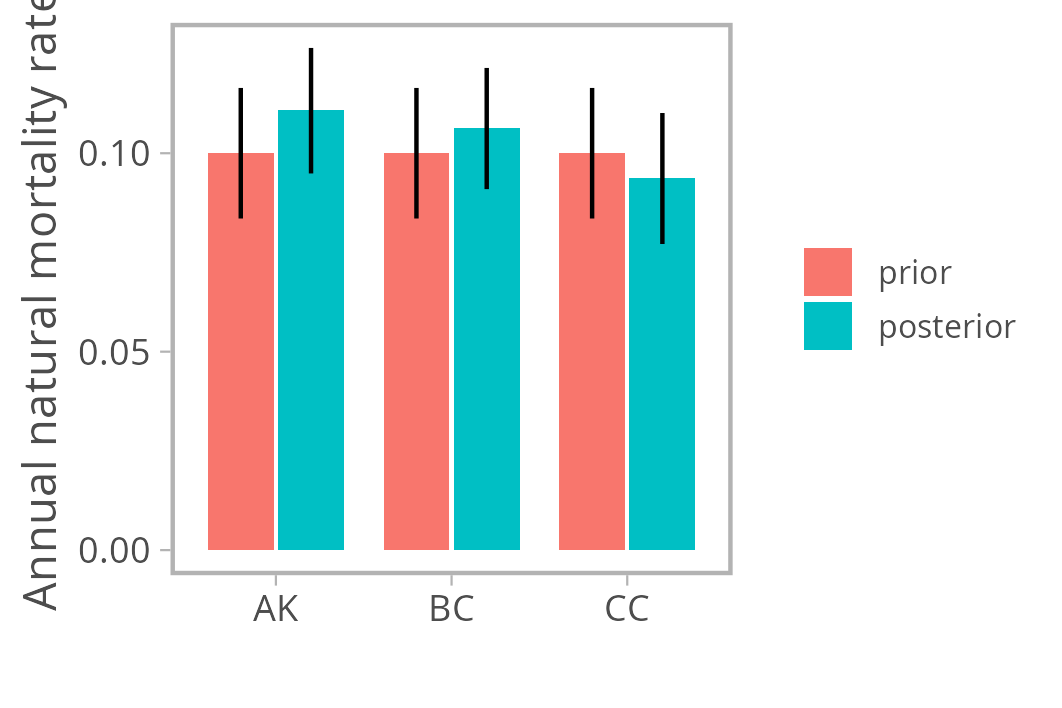
\includegraphics[width = 0.4\textwidth]{bar-regions-3-mortality-priors-posteriors}
    \caption{Sablefish annual natural mortality rate prior and posterior means (90\% CI) by jurisdiction. Orange bars: prior means; teal bars: posterior means. AK: Alaska; BC: British Columbia; CC: California Current.}
    \label{fig:bar-regions-3-mortality-priors-posteriors}
\end{figure}

\begin{figure}[htb]
    \centering
    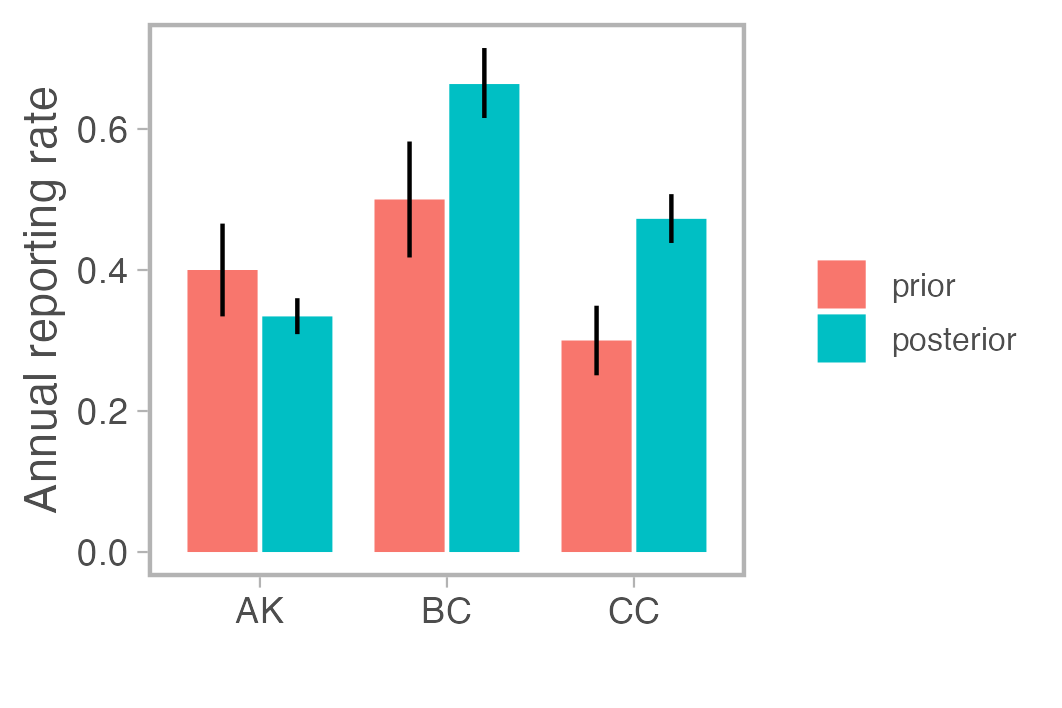
\includegraphics[width = 0.4\textwidth]{bar-regions-3-reporting-priors-posteriors}
    \caption{Sablefish annual tag reporting rate prior and posterior means (90\% CI) by jurisdiction. Orange bars: prior means; teal bars: posterior means. AK: Alaska; BC: British Columbia; CC: California Current.}
    \label{fig:bar-regions-3-reporting-priors-posteriors}
\end{figure}

\begin{figure}[htb]
    \centering
    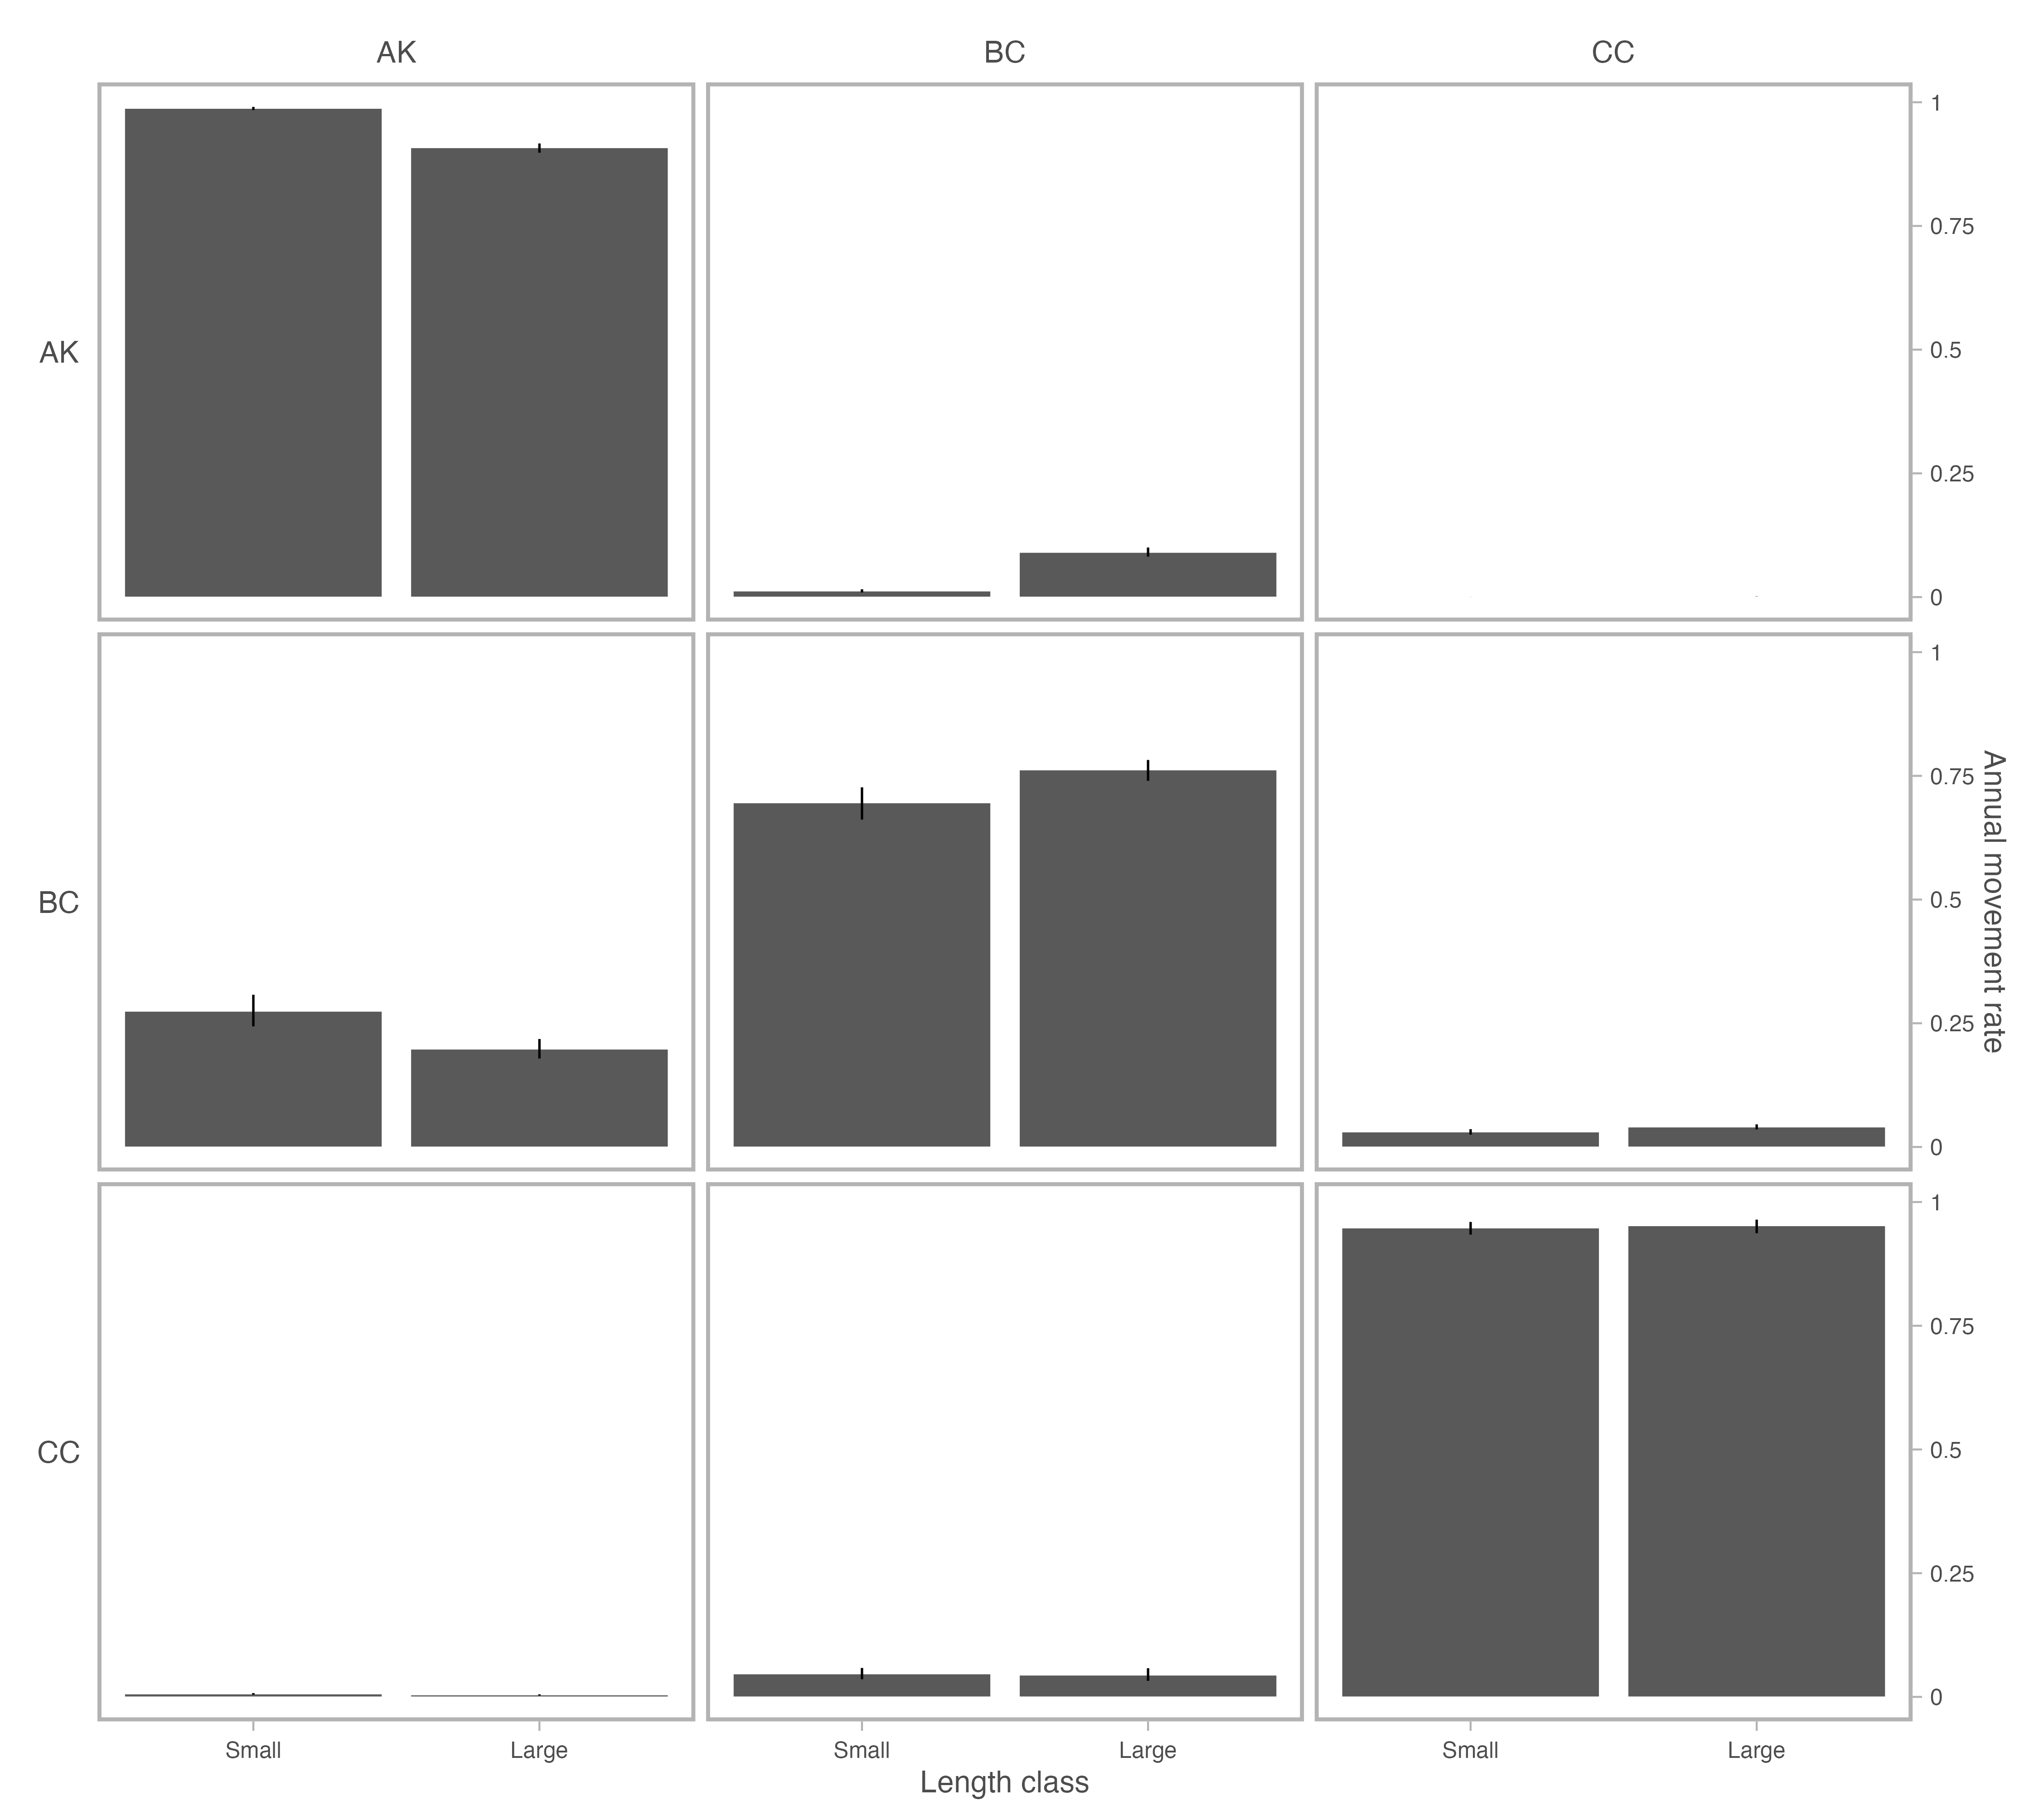
\includegraphics[width = 0.7\textwidth]{bar-regions-3-size}
    \caption{Sablefish mean annual movement rates (90\% CI) between three jurisdictions in the northeast Pacific Ocean by released size class. Panel rows: previous jurisdiction; panel columns: current jurisdiction. Small: fork length 400--549 mm; Large: fork length 550--800 mm. AK: Alaska; BC: British Columbia; CC: California Current.}
    \label{fig:bar-regions-3-size}
\end{figure}

\begin{figure}[htb]
    \centering
    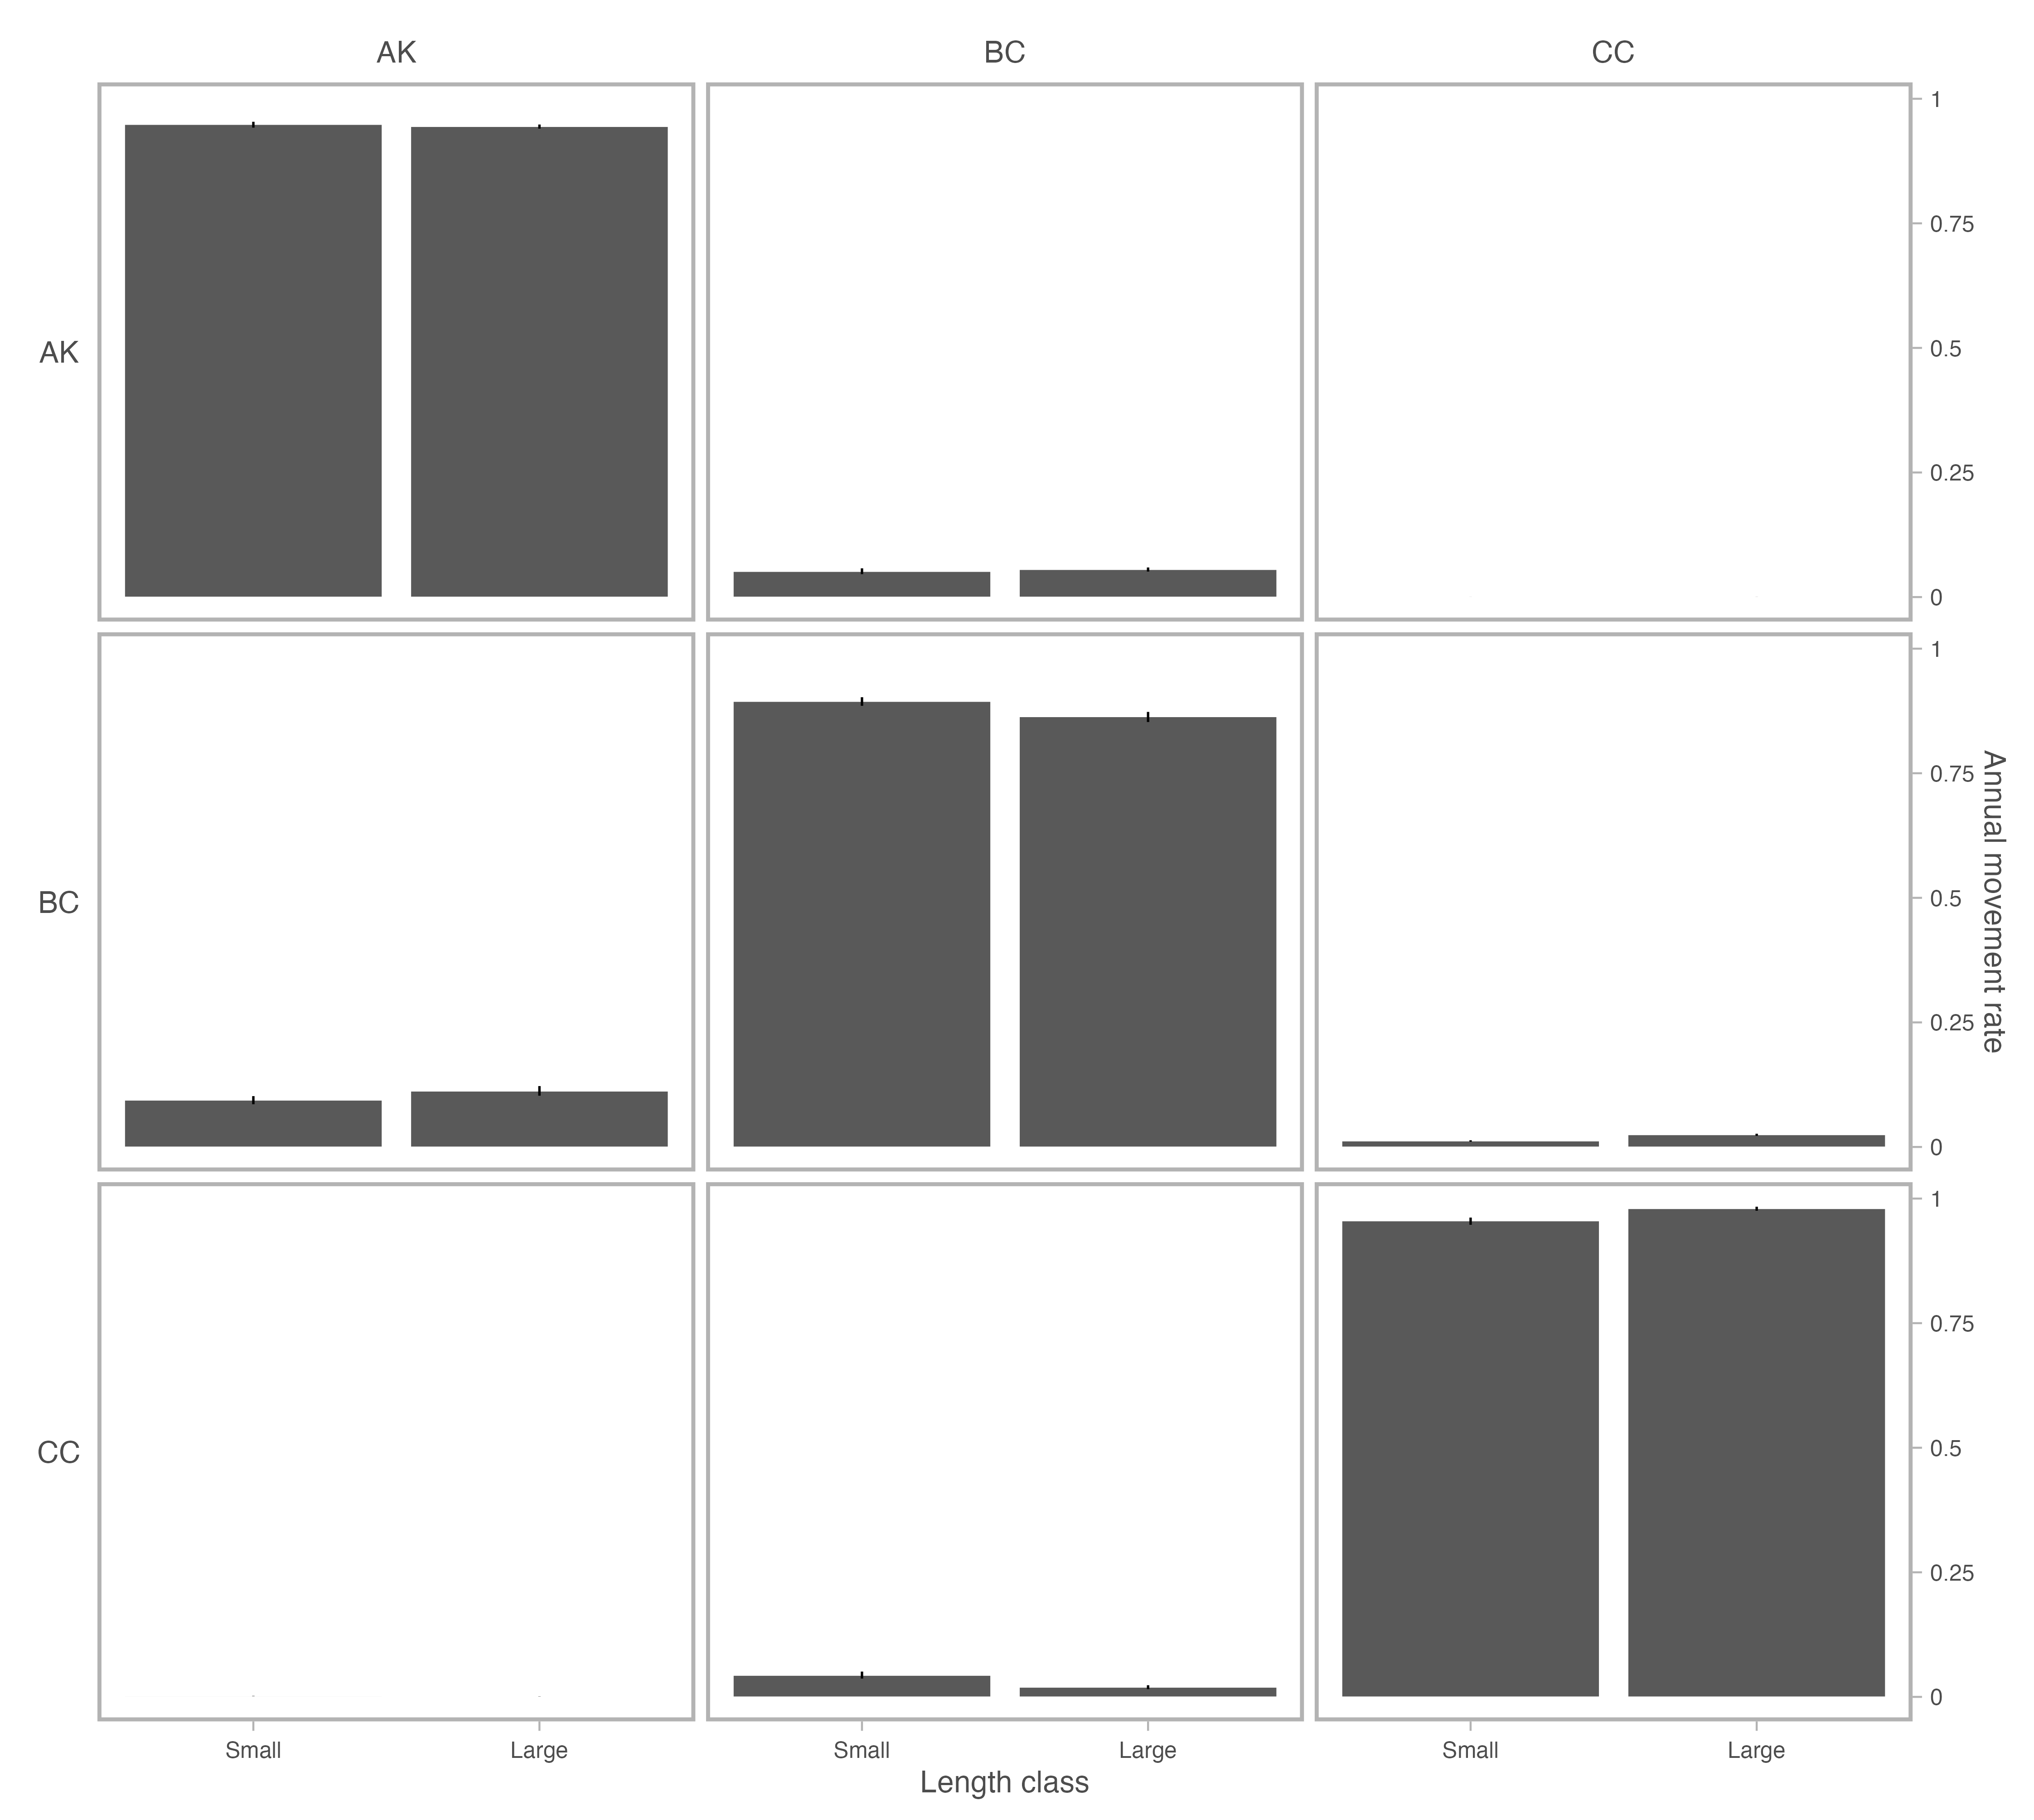
\includegraphics[width = 0.7\textwidth]{bar-regions-3-size-no-duration-constraint}
    \caption{TBD - No duration constraint - Suggest report change under no duration constraint as table}
    \label{fig:bar-regions-3-size-no-duration-constraint}
\end{figure}

\begin{figure}[htb]
    \centering
    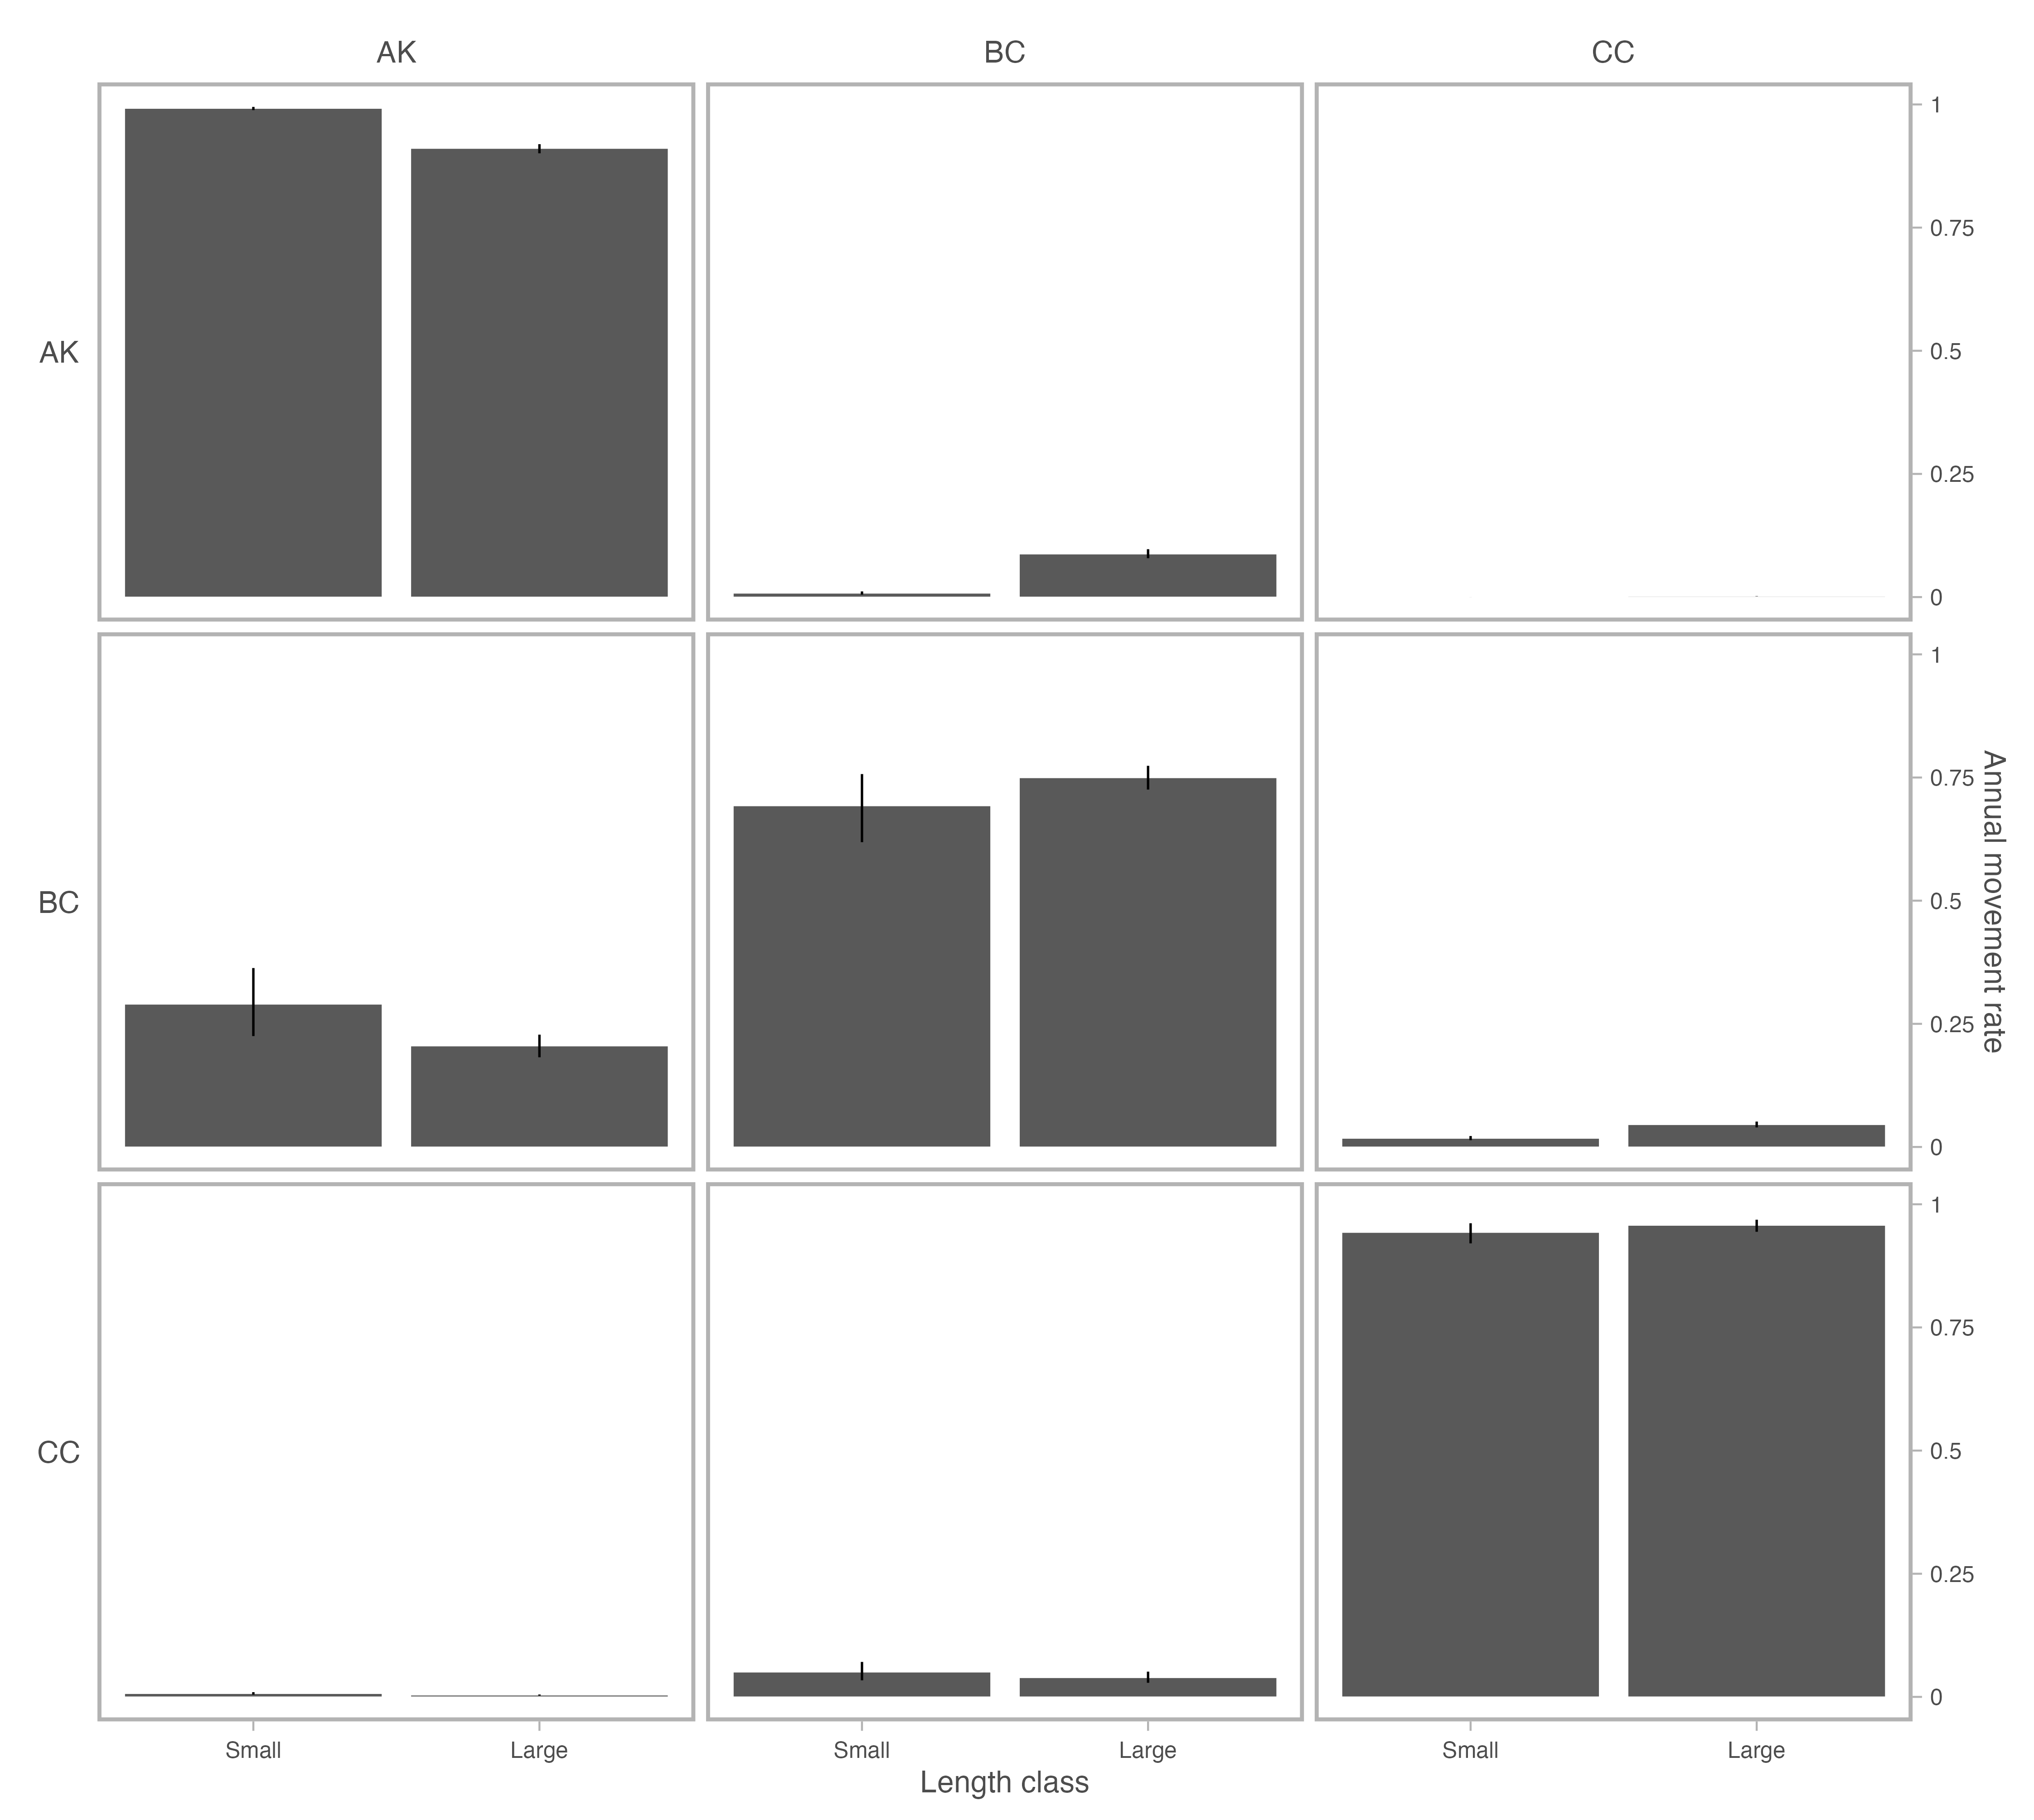
\includegraphics[width = 0.7\textwidth]{bar-regions-3-size-no-recovery-transition}
    \caption{TBD - No reocvery transition - Suggest report change under no recovery transition as table}
    \label{fig:bar-regions-3-size-no-recovery-transition}
\end{figure}

\begin{figure}[htb]
    \centering
    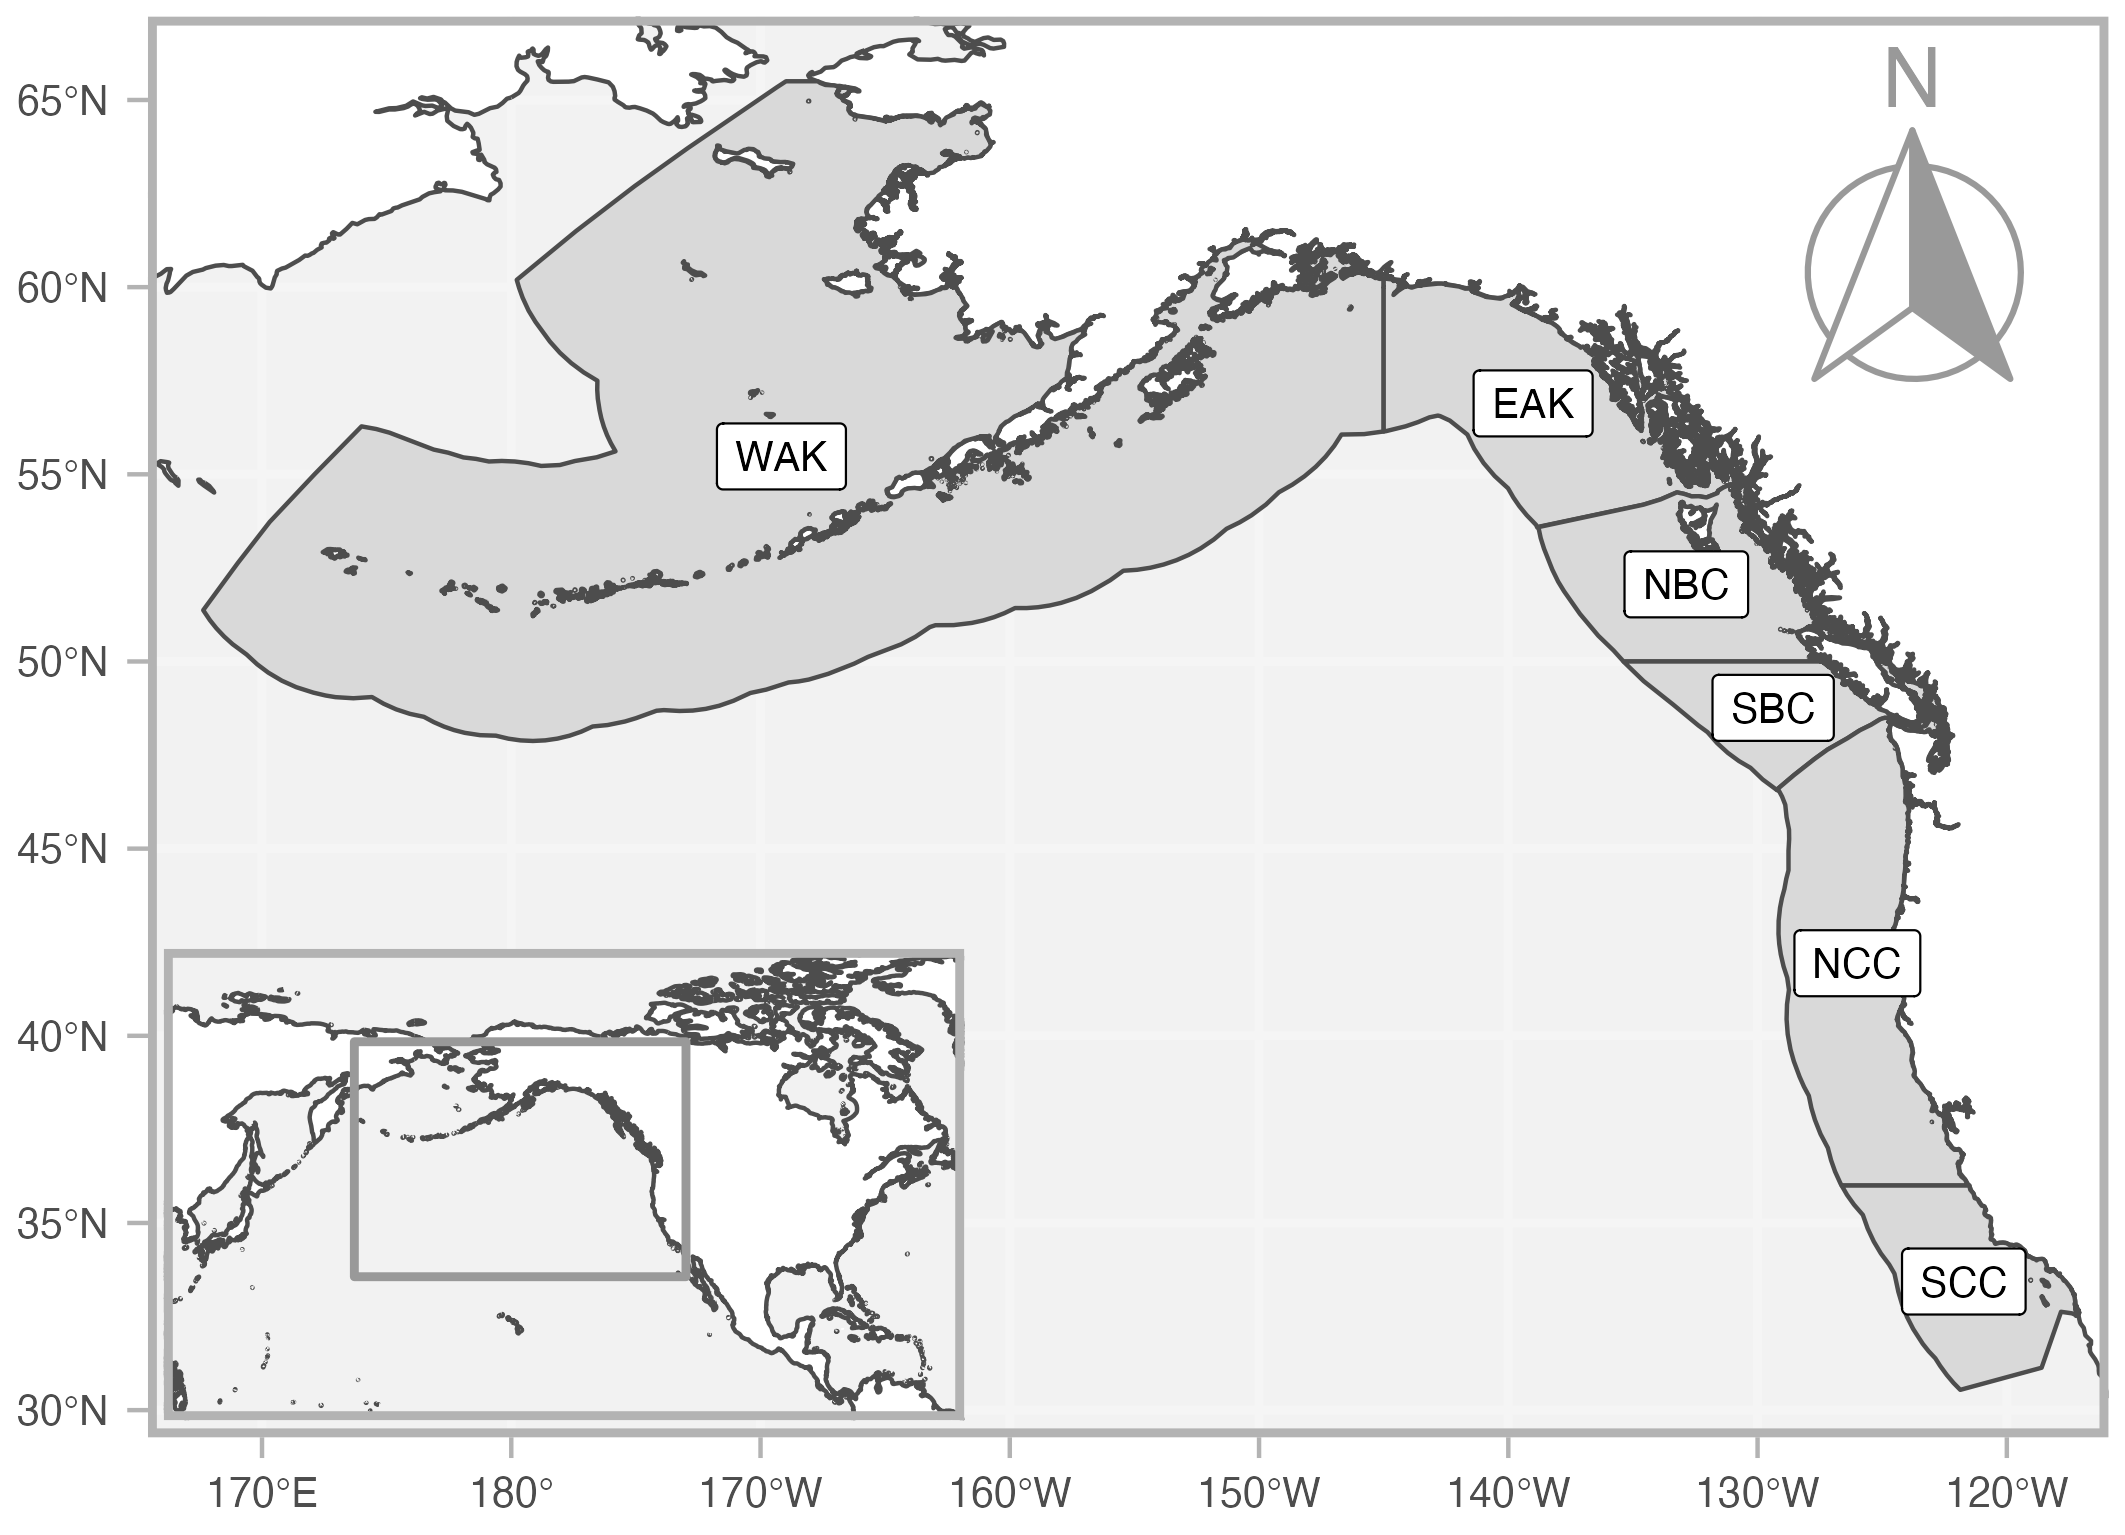
\includegraphics[width = 0.7\textwidth]{map-regions-6}
    \caption{Sablefish biogeographical regions in the northeast Pacific Ocean. WAK: West Alaska; EAK: East Alaska; NBC: North British Columbia; SBC: South British Columbia; NCC: North California Current; SCC: South California Current.}
    \label{fig:map-regions-6}
\end{figure}

\begin{figure}[htb]
    \centering
    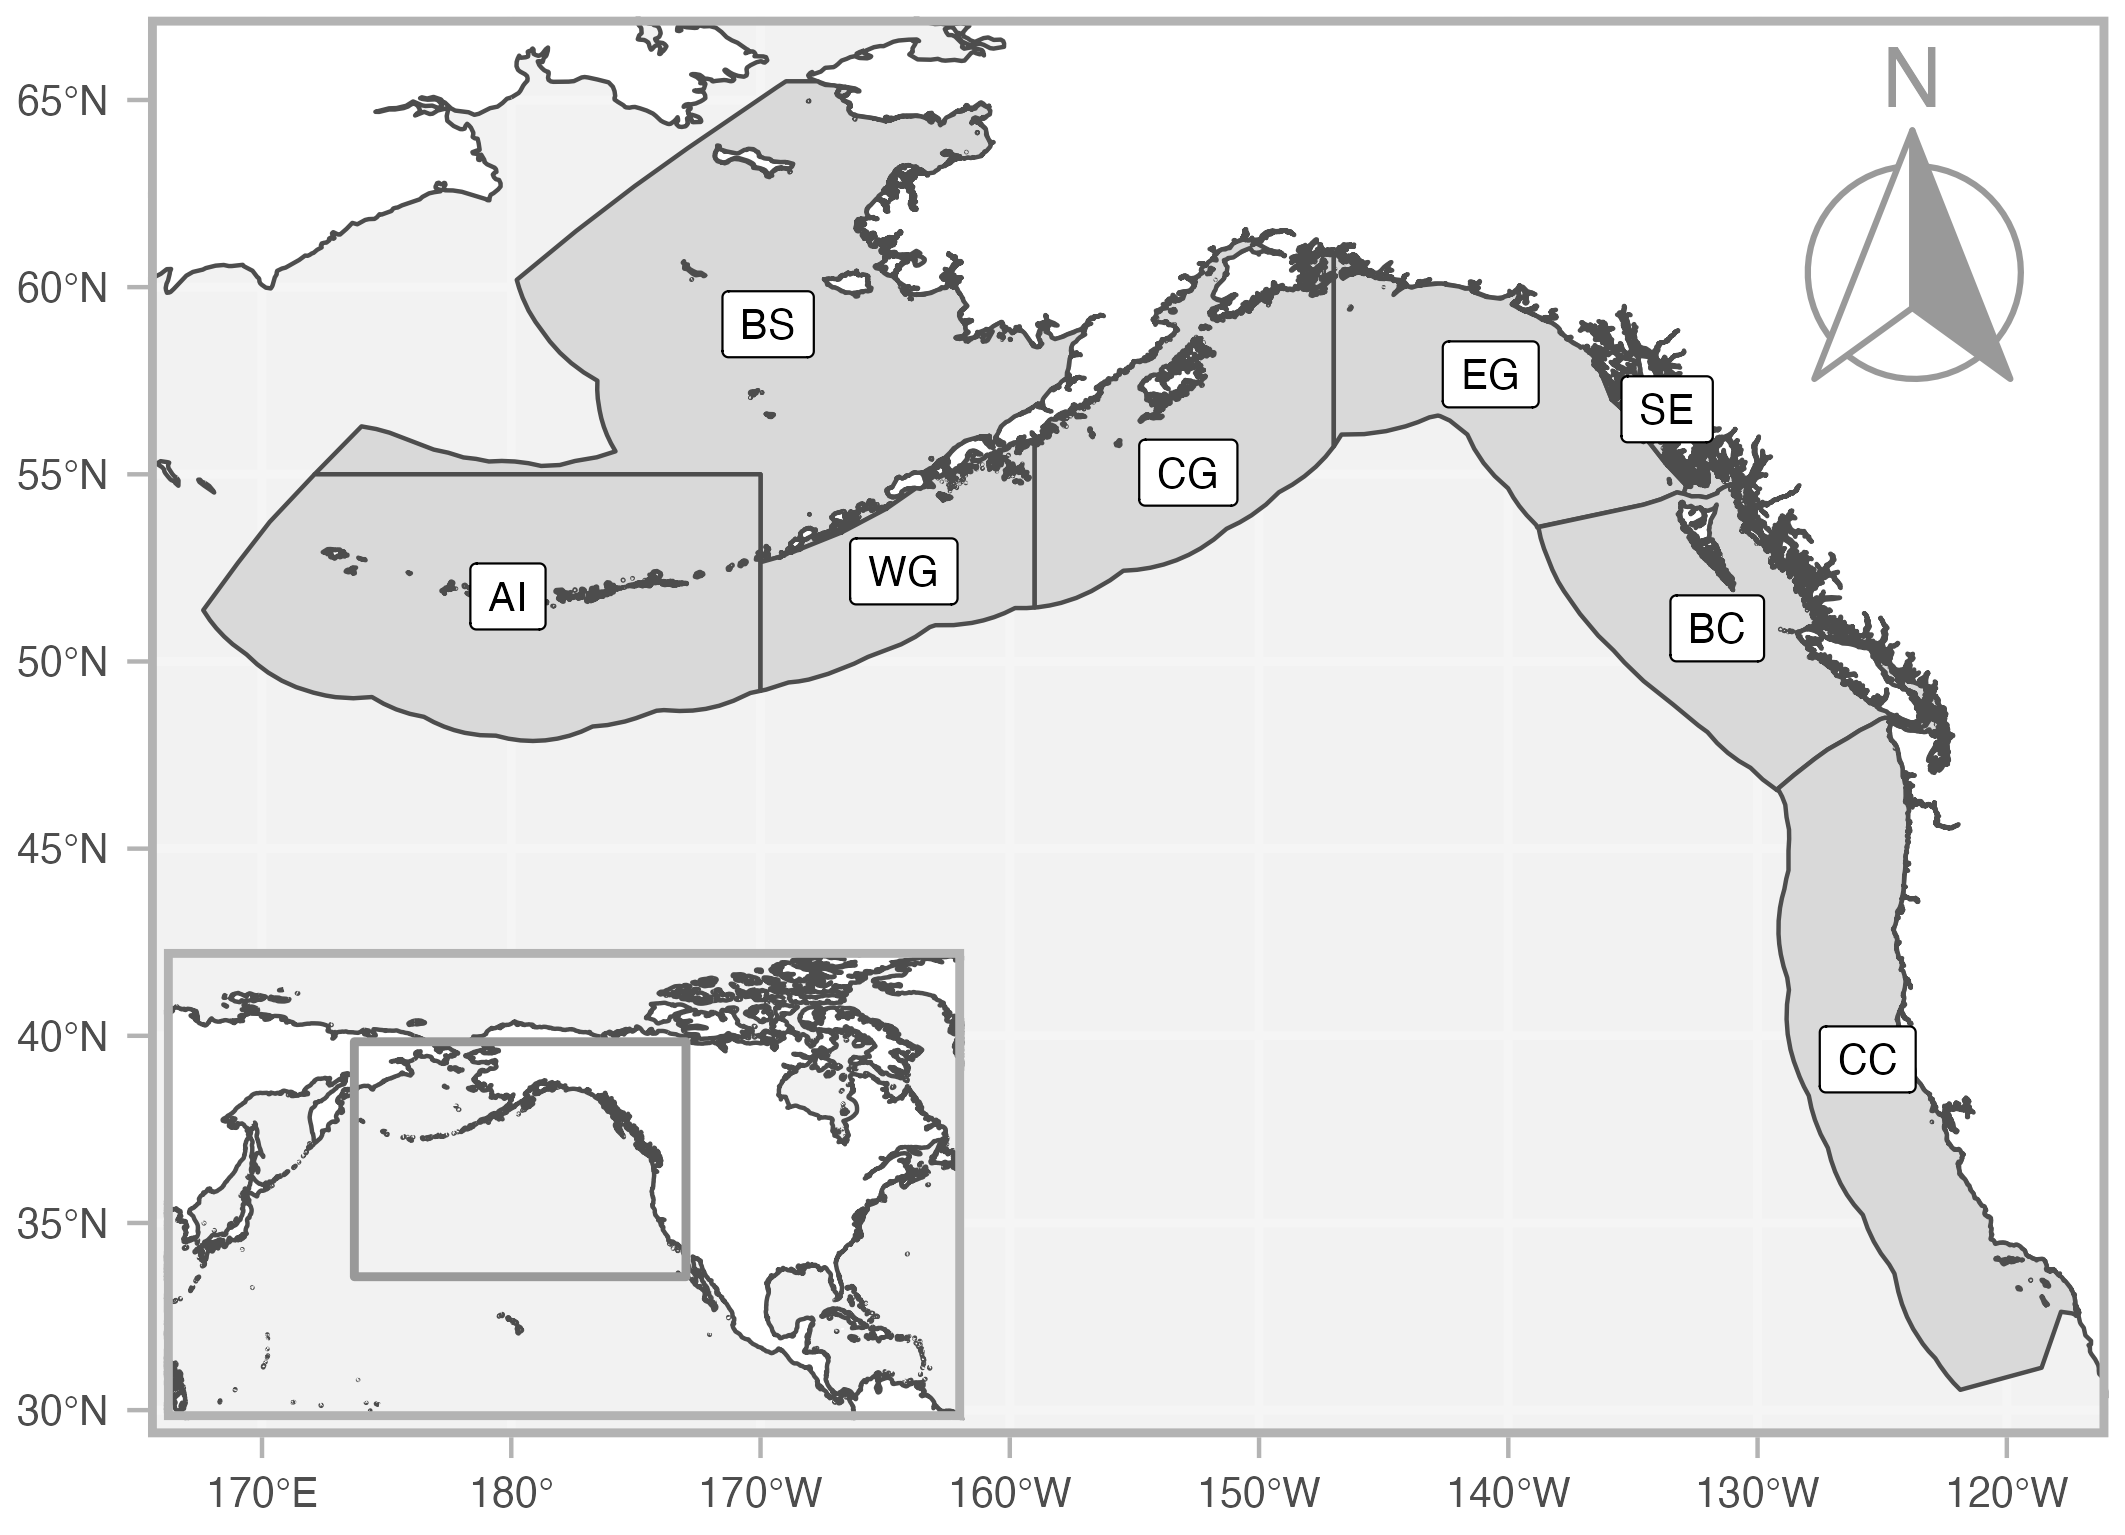
\includegraphics[width = 0.7\textwidth]{map-regions-8}
    \caption{Sablefish management regions in the northeast Pacific Ocean. BS: Bering Sea; AI: Aleutian Islands; WG: Western Gulf of Alaska; CG: Central Gulf of Alaska; EG: Eastern Gulf of Alaska; SE: Southeast Alaska; BC: British Columbia; CC: California Current.}
    \label{fig:map-regions-8}
\end{figure}


\subsection{Supplementary tables}

\begin{table}[h]
  \begin{center}
  \caption{Sablefish mean annual movement rates (per fish per year; 90\%{} CI) between three jurisdictions in the northeast Pacific Ocean. AK: Alaska; BC: British Columbia; CC: California Current.}
  \label{tab:movement-rate-regions-3-mean}
    \pgfplotstabletypeset[
      col sep=comma,                       % Commas separate .csv values
      columns/{0}/.style={column name={}}, % Replace autofilled column name by " "
      string type                          % Expect characters
    ]{tabs/movement-rate-regions-3-mean.csv}
  \end{center}
\end{table}

\begin{landscape}
\begin{table}[h]
  \begin{center}
  \caption{Sablefish mean annual movement rates (per fish per year; 90\%{} CI) between six biogeographic regions in the northeast Pacific Ocean. WAK: West Alaska; EAK: East Alaska; NBC: North British Columbia; SBC: South British Columbia; NCC: North California Current; SCC: South California Current.}
  \label{tab:movement-rate-regions-8-mean}
    \pgfplotstabletypeset[
      col sep=comma,                       % Commas separate .csv values
      columns/{0}/.style={column name={}}, % Replace autofilled column name by " "
      string type                          % Expect characters
    ]{tabs/movement-rate-regions-8-mean.csv}
  \end{center}
\end{table}
\end{landscape}

\begin{table}[h]
  \begin{center}
  \caption{TBD - 3x CV fishing rate - Consider reporting change as table}
  \label{tab:movement-rate-regions-3-mean-3x-cv-fishing-rate}
    \pgfplotstabletypeset[
      col sep=comma,                       % Commas separate .csv values
      columns/{0}/.style={column name={}}, % Replace autofilled column name by " "
      string type                          % Expect characters
    ]{tabs/movement-rate-regions-3-mean-3x-cv-fishing-rate.csv}
  \end{center}
\end{table}

\begin{table}[h]
  \begin{center}
  \caption{TBD - 3x sd reporting rate - Consider reporting change as table}
  \label{tab:movement-rate-regions-3-mean-3x-sd-reporting-rate}
    \pgfplotstabletypeset[
      col sep=comma,                       % Commas separate .csv values
      columns/{0}/.style={column name={}}, % Replace autofilled column name by " "
      string type                          % Expect characters
    ]{tabs/movement-rate-regions-3-mean-3x-sd-reporting-rate.csv}
  \end{center}
\end{table}

\begin{table}[h]
  \begin{center}
  \caption{Sablefish mean annual movement rates (per fish per year; 90\%{} CI) between three jurisdictions in the northeast Pacific Ocean for 1979--1994. AK: Alaska; BC: British Columbia; CC: California Current.}
%  \label{tab:movement-rate-regions-3-mean}
  \label{tab:movement-rate-regions-3-mean-block-1979-1994}
    \pgfplotstabletypeset[
      col sep=comma,                       % Commas separate .csv values
      columns/{0}/.style={column name={}}, % Replace autofilled column name by " "
      string type                          % Expect characters
    ]{tabs/movement-rate-regions-3-mean-block-1979-1994.csv}
  \end{center}
\end{table}

\begin{table}[h]
  \begin{center}
  \caption{Sablefish mean annual movement rates (per fish per year; 90\%{} CI) between three jurisdictions in the northeast Pacific Ocean for 1995--2006. AK: Alaska; BC: British Columbia; CC: California Current.}
%  \label{tab:movement-rate-regions-3-mean}
  \label{tab:movement-rate-regions-3-mean-block-1995-2006}
    \pgfplotstabletypeset[
      col sep=comma,                       % Commas separate .csv values
      columns/{0}/.style={column name={}}, % Replace autofilled column name by " "
      string type                          % Expect characters
    ]{tabs/movement-rate-regions-3-mean-block-1995-2006.csv}
  \end{center}
\end{table}

\begin{table}[h]
  \begin{center}
  \caption{Sablefish mean annual movement rates (per fish per year; 90\%{} CI) between three jurisdictions in the northeast Pacific Ocean for 2007--2017. AK: Alaska; BC: British Columbia; CC: California Current.}
%  \label{tab:movement-rate-regions-3-mean}
  \label{tab:movement-rate-regions-3-mean-block-2007-2017}
    \pgfplotstabletypeset[
      col sep=comma,                       % Commas separate .csv values
      columns/{0}/.style={column name={}}, % Replace autofilled column name by " "
      string type                          % Expect characters
    ]{tabs/movement-rate-regions-3-mean-block-2007-2017.csv}
  \end{center}
\end{table}


\newpage
\bibliography{refs}

% End
\end{document}








%%% Local Variables:
%%% mode: LaTeX
%%% TeX-master: t
%%% TeX-master: t
%%% End:
